%%%%%%%%%%%%%%%%%%%%%%%%%%%%%%%%%%%%%%%%%
% Masters/Doctoral Thesis
% LaTeX Template
% Version 2.5 (27/8/17)
%
% This template was downloaded from:
% http://www.LaTeXTemplates.com
%
% Version 2.x major modifications by:
% Vel (vel@latextemplates.com)
%
% This template is based on a template by:
% Steve Gunn (http://users.ecs.soton.ac.uk/srg/softwaretools/document/templates/)
% Sunil Patel (http://www.sunilpatel.co.uk/thesis-template/)
%
% Template license:
% CC BY-NC-SA 3.0 (http://creativecommons.org/licenses/by-nc-sa/3.0/)
%
%%%%%%%%%%%%%%%%%%%%%%%%%%%%%%%%%%%%%%%%%

%----------------------------------------------------------------------------------------
%	PACKAGES AND OTHER DOCUMENT CONFIGURATIONS
%----------------------------------------------------------------------------------------

\documentclass[
12pt, % The default document font size, options: 10pt, 11pt, 12pt
oneside, % Two side (alternating margins) for binding by default, uncomment to switch to one side
english, % ngerman for German
doublespacing, % Single line spacing, alternatives: onehalfspacing or doublespacing
%draft, % Uncomment to enable draft mode (no pictures, no links, overfull hboxes indicated)
%nolistspacing, % If the document is onehalfspacing or doublespacing, uncomment this to set spacing in lists to single
%liststotoc, % Uncomment to add the list of figures/tables/etc to the table of contents
%toctotoc, % Uncomment to add the main table of contents to the table of contents
%parskip, % Uncomment to add space between paragraphs
%nohyperref, % Uncomment to not load the hyperref package
headsepline, % Uncomment to get a line under the header
%chapterinoneline, % Uncomment to place the chapter title next to the number on one line
%consistentlayout, % Uncomment to change the layout of the declaration, abstract and acknowledgements pages to match the default layout
]{MastersDoctoralThesis} % The class file specifying the document structure

\usepackage[utf8]{inputenc} % Required for inputting international characters
\usepackage[T1]{fontenc} % Output font encoding for international characters
\usepackage{subcaption}
\usepackage{mathpazo} % Use the Palatino font by default
\usepackage[colorinlistoftodos]{todonotes}
\usepackage{booktabs}
\usepackage{colortbl}
\usepackage{xcolor}
\usepackage[backend=bibtex,style=authoryear,natbib=true]{biblatex} % Use the bibtex backend with the authoryear citation style (which resembles APA)

\addbibresource{example.bib} % The filename of the bibliography
\addbibresource{Zotero.bib}

\usepackage[autostyle=true]{csquotes} % Required to generate language-dependent quotes in the bibliography

%----------------------------------------------------------------------------------------
%	MARGIN SETTINGS
%----------------------------------------------------------------------------------------

\geometry{
	paper=a4paper, % Change to letterpaper for US letter
	inner=2.5cm, % Inner margin
	outer=3.8cm, % Outer margin
	bindingoffset=.5cm, % Binding offset
	top=1.5cm, % Top margin
	bottom=1.5cm, % Bottom margin
	%showframe, % Uncomment to show how the type block is set on the page
}

%----------------------------------------------------------------------------------------
%	THESIS INFORMATION
%----------------------------------------------------------------------------------------

\thesistitle{Building an Interface for Haptic Spatial Navigation} % Your thesis title, this is used in the title and abstract, print it elsewhere with \ttitle
\supervisor{Dr. Simon \textsc{Perrault}} % Your supervisor's name, this is used in the title page, print it elsewhere with \supname
\examiner{Dr. David A. \textsc{Smith}} % Your examiner's name, this is not currently used anywhere in the template, print it elsewhere with \examname
\degree{B.Sc (Hons)} % Your degree name, this is used in the title page and abstract, print it elsewhere with \degreename
\author{Hrishi \textsc{Olickel}} % Your name, this is used in the title page and abstract, print it elsewhere with \authorname
\addresses{} % Your address, this is not currently used anywhere in the template, print it elsewhere with \addressname

\subject{Mathematical, Computational and Statistical Sciences} % Your subject area, this is not currently used anywhere in the template, print it elsewhere with \subjectname
\keywords{} % Keywords for your thesis, this is not currently used anywhere in the template, print it elsewhere with \keywordnames
\university{\href{https://www.yale-nus.edu.sg/}{Yale-NUS College}} % Your university's name and URL, this is used in the title page and abstract, print it elsewhere with \univname
\department{{}} % Your department's name and URL, this is used in the title page and abstract, print it elsewhere with \deptname
\group{{}} % Your research group's name and URL, this is used in the title page, print it elsewhere with \groupname
\faculty{{}} % Your faculty's name and URL, this is used in the title page and abstract, print it elsewhere with \facname

\AtBeginDocument{
\hypersetup{colorlinks=false}
\hypersetup{pdftitle=\ttitle} % Set the PDF's title to your title
\hypersetup{pdfauthor=\authorname} % Set the PDF's author to your name
\hypersetup{pdfkeywords=\keywordnames} % Set the PDF's keywords to your keywords
}

\begin{document}

\frontmatter % Use roman page numbering style (i, ii, iii, iv...) for the pre-content pages

\pagestyle{plain} % Default to the plain heading style until the thesis style is called for the body content

%----------------------------------------------------------------------------------------
%	TITLE PAGE
%----------------------------------------------------------------------------------------

\begin{titlepage}
\begin{center}

\vspace*{.06\textheight}
{\scshape\LARGE \univname\par}\vspace{1.5cm} % University name
\textsc{\Large Capstone Report}\\[0.5cm] % Thesis type

\HRule \\[0.4cm] % Horizontal line
{\huge \bfseries \ttitle\par}\vspace{0.4cm} % Thesis title
\HRule \\[1.5cm] % Horizontal line

\begin{minipage}[t]{0.4\textwidth}
\begin{flushleft} \large
\emph{Author:}\\
{\authorname} % Author name - remove the \href bracket to remove the link
\end{flushleft}
\end{minipage}
\begin{minipage}[t]{0.4\textwidth}
\begin{flushright} \large
\emph{Supervisor:} \\
{\supname} % Supervisor name - remove the \href bracket to remove the link
\end{flushright}
\end{minipage}\\[3cm]

\vfill

\large \textit{A thesis submitted in fulfillment of the requirements\\ for the degree of \degreename}\\[0.3cm] % University requirement text
% \textit{in the}\\[0.4cm]
% \groupname\\\deptname\\[2cm] % Research group name and department name

\vfill

{\large \today}\\[4cm] % Date
%\includegraphics{Logo} % University/department logo - uncomment to place it

\vfill
\end{center}
\end{titlepage}

%----------------------------------------------------------------------------------------
%	DECLARATION PAGE
%----------------------------------------------------------------------------------------

\begin{declaration}
\addchaptertocentry{\authorshipname} % Add the declaration to the table of contents

\noindent I, \authorname, declare that the product of this Project, the Thesis, is the end result of my own work and that due acknowledgement has been given in the bibliography and references to ALL sources be they  printed, electronic, or personal, in accordance with the academic regulations of Yale‐NUS College.

% I confirm that:
%
% \begin{itemize}
% \item This work was done wholly or mainly while in candidature for a research degree at this University.
% \item Where any part of this thesis has previously been submitted for a degree or any other qualification at this University or any other institution, this has been clearly stated.
% \item Where I have consulted the published work of others, this is always clearly attributed.
% \item Where I have quoted from the work of others, the source is always given. With the exception of such quotations, this thesis is entirely my own work.
% \item I have acknowledged all main sources of help.
% \item Where the thesis is based on work done by myself jointly with others, I have made clear exactly what was done by others and what I have contributed myself.\\
% \end{itemize}

\noindent Signed:\\
\rule[0.5em]{25em}{0.5pt} % This prints a line for the signature

\noindent Date:\\
\rule[0.5em]{25em}{0.5pt} % This prints a line to write the date
\end{declaration}

\cleardoublepage

%----------------------------------------------------------------------------------------
%	QUOTATION PAGE
%----------------------------------------------------------------------------------------

% \vspace*{0.2\textheight}
%
% \noindent\enquote{\itshape Thanks to my solid academic training, today I can write hundreds of words on virtually any topic without possessing a shred of information, which is how I got a good job in journalism.}\bigbreak
%
% \hfill Dave Barry

%----------------------------------------------------------------------------------------
%	ABSTRACT PAGE
%----------------------------------------------------------------------------------------

\begin{abstract}
\addchaptertocentry{\abstractname} % Add the abstract to the table of contents
Sensory substitution is a field of Human Computer Interaction that has long been explored as a possible avenue to replace and improve human sensory perception. This paper explores novel frameworks for designing and evaluating a sensory substitution system based on haptic feedback, in a way that can build a standard extensible base for future research. A new device for haptic spatial navigation, along with a novel encoding protocol is also developed, and evaluated. Results show that training is a signifcant component of such systems, as well as indicating possible features that can improve the experience of the user.
\end{abstract}

%----------------------------------------------------------------------------------------
%	ACKNOWLEDGEMENTS
%----------------------------------------------------------------------------------------

\begin{acknowledgements}
\addchaptertocentry{\acknowledgementname} % Add the acknowledgements to the table of contents

I would like to thank my capstone supervisor Prof. Simon Perrault for the invaluable guidance in shaping what was a weekend project into a capstone thesis, and for helping me through the many, many obstacles along the way. This project would not have the form it does today without his constant support and valued feedback.

I would also like to thank Aaron Ong and Parag Bhatnagar for help in developing the kernel that was haptic sensory substitution into a real project, and for the apt criticism and many midnights spent poring over the viability of the prototypes.

I am very thankful to my capstone examiner, Prof. David Smith, whose contributions both in writing and in person to this report have made it (by multiple accounts) far more understandable yet succinct.

I am extremely grateful for the MCS batch of 2018, whose support and camaraderie in the tough times of the year helped complete this project, and keep me sane as I write the final sentences of it.

I would also like to thank all the participants that made time for the experiment even as it was uncompensated, and stayed seated in a chair in my room, in the blind for much time as I fumbled about trying to reset the experiment.

Finally, I'd like to thank Hebe Hilhorst for her sharp quick-witted criticism and warm support from the very inception of this project. I could not have done it without you.

\end{acknowledgements}

%----------------------------------------------------------------------------------------
%	LIST OF CONTENTS/FIGURES/TABLES PAGES
%----------------------------------------------------------------------------------------

\tableofcontents % Prints the main table of contents

\listoffigures % Prints the list of figures

\listoftables % Prints the list of tables

%----------------------------------------------------------------------------------------
%	ABBREVIATIONS
%----------------------------------------------------------------------------------------

% \begin{abbreviations}{ll} % Include a list of abbreviations (a table of two columns)
%
% \textbf{LAH} & \textbf{L}ist \textbf{A}bbreviations \textbf{H}ere\\
% \textbf{WSF} & \textbf{W}hat (it) \textbf{S}tands \textbf{F}or\\
%
% \end{abbreviations}

%----------------------------------------------------------------------------------------
%	PHYSICAL CONSTANTS/OTHER DEFINITIONS
%----------------------------------------------------------------------------------------

% \begin{constants}{lr@{${}={}$}l} % The list of physical constants is a three column table
%
% % The \SI{}{} command is provided by the siunitx package, see its documentation for instructions on how to use it
%
% Speed of Light & $c_{0}$ & \SI{2.99792458e8}{\meter\per\second} (exact)\\
% %Constant Name & $Symbol$ & $Constant Value$ with units\\
%
% \end{constants}

%----------------------------------------------------------------------------------------
%	SYMBOLS
%----------------------------------------------------------------------------------------

% \begin{symbols}{lll} % Include a list of Symbols (a three column table)
%
% $a$ & distance & \si{\meter} \\
% $P$ & power & \si{\watt} (\si{\joule\per\second}) \\
% %Symbol & Name & Unit \\
%
% \addlinespace % Gap to separate the Roman symbols from the Greek
%
% $\omega$ & angular frequency & \si{\radian} \\
%
% \end{symbols}

%----------------------------------------------------------------------------------------
%	DEDICATION
%----------------------------------------------------------------------------------------

% \dedicatory{For/Dedicated to/To my\ldots}

%----------------------------------------------------------------------------------------
%	THESIS CONTENT - CHAPTERS
%----------------------------------------------------------------------------------------

\mainmatter % Begin numeric (1,2,3...) page numbering

\pagestyle{thesis} % Return the page headers back to the "thesis" style

% Include the chapters of the thesis as separate files from the Chapters folder
% Uncomment the lines as you write the chapters

% % Chapter 1

\chapter{Chapter Title Here} % Main chapter title

\label{Chapter1} % For referencing the chapter elsewhere, use \ref{Chapter1} 

%----------------------------------------------------------------------------------------

% Define some commands to keep the formatting separated from the content 
\newcommand{\keyword}[1]{\textbf{#1}}
\newcommand{\tabhead}[1]{\textbf{#1}}
\newcommand{\code}[1]{\texttt{#1}}
\newcommand{\file}[1]{\texttt{\bfseries#1}}
\newcommand{\option}[1]{\texttt{\itshape#1}}

%----------------------------------------------------------------------------------------

\section{Welcome and Thank You}
Welcome to this \LaTeX{} Thesis Template, a beautiful and easy to use template for writing a thesis using the \LaTeX{} typesetting system.

If you are writing a thesis (or will be in the future) and its subject is technical or mathematical (though it doesn't have to be), then creating it in \LaTeX{} is highly recommended as a way to make sure you can just get down to the essential writing without having to worry over formatting or wasting time arguing with your word processor.

\LaTeX{} is easily able to professionally typeset documents that run to hundreds or thousands of pages long. With simple mark-up commands, it automatically sets out the table of contents, margins, page headers and footers and keeps the formatting consistent and beautiful. One of its main strengths is the way it can easily typeset mathematics, even \emph{heavy} mathematics. Even if those equations are the most horribly twisted and most difficult mathematical problems that can only be solved on a super-computer, you can at least count on \LaTeX{} to make them look stunning.

%----------------------------------------------------------------------------------------

\section{Learning \LaTeX{}}

\LaTeX{} is not a \textsc{wysiwyg} (What You See is What You Get) program, unlike word processors such as Microsoft Word or Apple's Pages. Instead, a document written for \LaTeX{} is actually a simple, plain text file that contains \emph{no formatting}. You tell \LaTeX{} how you want the formatting in the finished document by writing in simple commands amongst the text, for example, if I want to use \emph{italic text for emphasis}, I write the \verb|\emph{text}| command and put the text I want in italics in between the curly braces. This means that \LaTeX{} is a \enquote{mark-up} language, very much like HTML.

\subsection{A (not so short) Introduction to \LaTeX{}}

If you are new to \LaTeX{}, there is a very good eBook -- freely available online as a PDF file -- called, \enquote{The Not So Short Introduction to \LaTeX{}}. The book's title is typically shortened to just \emph{lshort}. You can download the latest version (as it is occasionally updated) from here:
\url{http://www.ctan.org/tex-archive/info/lshort/english/lshort.pdf}

It is also available in several other languages. Find yours from the list on this page: \url{http://www.ctan.org/tex-archive/info/lshort/}

It is recommended to take a little time out to learn how to use \LaTeX{} by creating several, small `test' documents, or having a close look at several templates on:\\ 
\url{http://www.LaTeXTemplates.com}\\ 
Making the effort now means you're not stuck learning the system when what you \emph{really} need to be doing is writing your thesis.

\subsection{A Short Math Guide for \LaTeX{}}

If you are writing a technical or mathematical thesis, then you may want to read the document by the AMS (American Mathematical Society) called, \enquote{A Short Math Guide for \LaTeX{}}. It can be found online here:
\url{http://www.ams.org/tex/amslatex.html}
under the \enquote{Additional Documentation} section towards the bottom of the page.

\subsection{Common \LaTeX{} Math Symbols}
There are a multitude of mathematical symbols available for \LaTeX{} and it would take a great effort to learn the commands for them all. The most common ones you are likely to use are shown on this page:
\url{http://www.sunilpatel.co.uk/latex-type/latex-math-symbols/}

You can use this page as a reference or crib sheet, the symbols are rendered as large, high quality images so you can quickly find the \LaTeX{} command for the symbol you need.

\subsection{\LaTeX{} on a Mac}
 
The \LaTeX{} distribution is available for many systems including Windows, Linux and Mac OS X. The package for OS X is called MacTeX and it contains all the applications you need -- bundled together and pre-customized -- for a fully working \LaTeX{} environment and work flow.
 
MacTeX includes a custom dedicated \LaTeX{} editor called TeXShop for writing your `\file{.tex}' files and BibDesk: a program to manage your references and create your bibliography section just as easily as managing songs and creating playlists in iTunes.

%----------------------------------------------------------------------------------------

\section{Getting Started with this Template}

If you are familiar with \LaTeX{}, then you should explore the directory structure of the template and then proceed to place your own information into the \emph{THESIS INFORMATION} block of the \file{main.tex} file. You can then modify the rest of this file to your unique specifications based on your degree/university. Section \ref{FillingFile} on page \pageref{FillingFile} will help you do this. Make sure you also read section \ref{ThesisConventions} about thesis conventions to get the most out of this template.

If you are new to \LaTeX{} it is recommended that you carry on reading through the rest of the information in this document.

Before you begin using this template you should ensure that its style complies with the thesis style guidelines imposed by your institution. In most cases this template style and layout will be suitable. If it is not, it may only require a small change to bring the template in line with your institution's recommendations. These modifications will need to be done on the \file{MastersDoctoralThesis.cls} file.

\subsection{About this Template}

This \LaTeX{} Thesis Template is originally based and created around a \LaTeX{} style file created by Steve R.\ Gunn from the University of Southampton (UK), department of Electronics and Computer Science. You can find his original thesis style file at his site, here:
\url{http://www.ecs.soton.ac.uk/~srg/softwaretools/document/templates/}

Steve's \file{ecsthesis.cls} was then taken by Sunil Patel who modified it by creating a skeleton framework and folder structure to place the thesis files in. The resulting template can be found on Sunil's site here:
\url{http://www.sunilpatel.co.uk/thesis-template}

Sunil's template was made available through \url{http://www.LaTeXTemplates.com} where it was modified many times based on user requests and questions. Version 2.0 and onwards of this template represents a major modification to Sunil's template and is, in fact, hardly recognisable. The work to make version 2.0 possible was carried out by \href{mailto:vel@latextemplates.com}{Vel} and Johannes Böttcher.

%----------------------------------------------------------------------------------------

\section{What this Template Includes}

\subsection{Folders}

This template comes as a single zip file that expands out to several files and folders. The folder names are mostly self-explanatory:

\keyword{Appendices} -- this is the folder where you put the appendices. Each appendix should go into its own separate \file{.tex} file. An example and template are included in the directory.

\keyword{Chapters} -- this is the folder where you put the thesis chapters. A thesis usually has about six chapters, though there is no hard rule on this. Each chapter should go in its own separate \file{.tex} file and they can be split as:
\begin{itemize}
\item Chapter 1: Introduction to the thesis topic
\item Chapter 2: Background information and theory
\item Chapter 3: (Laboratory) experimental setup
\item Chapter 4: Details of experiment 1
\item Chapter 5: Details of experiment 2
\item Chapter 6: Discussion of the experimental results
\item Chapter 7: Conclusion and future directions
\end{itemize}
This chapter layout is specialised for the experimental sciences, your discipline may be different.

\keyword{Figures} -- this folder contains all figures for the thesis. These are the final images that will go into the thesis document.

\subsection{Files}

Included are also several files, most of them are plain text and you can see their contents in a text editor. After initial compilation, you will see that more auxiliary files are created by \LaTeX{} or BibTeX and which you don't need to delete or worry about:

\keyword{example.bib} -- this is an important file that contains all the bibliographic information and references that you will be citing in the thesis for use with BibTeX. You can write it manually, but there are reference manager programs available that will create and manage it for you. Bibliographies in \LaTeX{} are a large subject and you may need to read about BibTeX before starting with this. Many modern reference managers will allow you to export your references in BibTeX format which greatly eases the amount of work you have to do.

\keyword{MastersDoctoralThesis.cls} -- this is an important file. It is the class file that tells \LaTeX{} how to format the thesis. 

\keyword{main.pdf} -- this is your beautifully typeset thesis (in the PDF file format) created by \LaTeX{}. It is supplied in the PDF with the template and after you compile the template you should get an identical version.

\keyword{main.tex} -- this is an important file. This is the file that you tell \LaTeX{} to compile to produce your thesis as a PDF file. It contains the framework and constructs that tell \LaTeX{} how to layout the thesis. It is heavily commented so you can read exactly what each line of code does and why it is there. After you put your own information into the \emph{THESIS INFORMATION} block -- you have now started your thesis!

Files that are \emph{not} included, but are created by \LaTeX{} as auxiliary files include:

\keyword{main.aux} -- this is an auxiliary file generated by \LaTeX{}, if it is deleted \LaTeX{} simply regenerates it when you run the main \file{.tex} file.

\keyword{main.bbl} -- this is an auxiliary file generated by BibTeX, if it is deleted, BibTeX simply regenerates it when you run the \file{main.aux} file. Whereas the \file{.bib} file contains all the references you have, this \file{.bbl} file contains the references you have actually cited in the thesis and is used to build the bibliography section of the thesis.

\keyword{main.blg} -- this is an auxiliary file generated by BibTeX, if it is deleted BibTeX simply regenerates it when you run the main \file{.aux} file.

\keyword{main.lof} -- this is an auxiliary file generated by \LaTeX{}, if it is deleted \LaTeX{} simply regenerates it when you run the main \file{.tex} file. It tells \LaTeX{} how to build the \emph{List of Figures} section.

\keyword{main.log} -- this is an auxiliary file generated by \LaTeX{}, if it is deleted \LaTeX{} simply regenerates it when you run the main \file{.tex} file. It contains messages from \LaTeX{}, if you receive errors and warnings from \LaTeX{}, they will be in this \file{.log} file.

\keyword{main.lot} -- this is an auxiliary file generated by \LaTeX{}, if it is deleted \LaTeX{} simply regenerates it when you run the main \file{.tex} file. It tells \LaTeX{} how to build the \emph{List of Tables} section.

\keyword{main.out} -- this is an auxiliary file generated by \LaTeX{}, if it is deleted \LaTeX{} simply regenerates it when you run the main \file{.tex} file.

So from this long list, only the files with the \file{.bib}, \file{.cls} and \file{.tex} extensions are the most important ones. The other auxiliary files can be ignored or deleted as \LaTeX{} and BibTeX will regenerate them.

%----------------------------------------------------------------------------------------

\section{Filling in Your Information in the \file{main.tex} File}\label{FillingFile}

You will need to personalise the thesis template and make it your own by filling in your own information. This is done by editing the \file{main.tex} file in a text editor or your favourite LaTeX environment.

Open the file and scroll down to the third large block titled \emph{THESIS INFORMATION} where you can see the entries for \emph{University Name}, \emph{Department Name}, etc \ldots

Fill out the information about yourself, your group and institution. You can also insert web links, if you do, make sure you use the full URL, including the \code{http://} for this. If you don't want these to be linked, simply remove the \verb|\href{url}{name}| and only leave the name.

When you have done this, save the file and recompile \code{main.tex}. All the information you filled in should now be in the PDF, complete with web links. You can now begin your thesis proper!

%----------------------------------------------------------------------------------------

\section{The \code{main.tex} File Explained}

The \file{main.tex} file contains the structure of the thesis. There are plenty of written comments that explain what pages, sections and formatting the \LaTeX{} code is creating. Each major document element is divided into commented blocks with titles in all capitals to make it obvious what the following bit of code is doing. Initially there seems to be a lot of \LaTeX{} code, but this is all formatting, and it has all been taken care of so you don't have to do it.

Begin by checking that your information on the title page is correct. For the thesis declaration, your institution may insist on something different than the text given. If this is the case, just replace what you see with what is required in the \emph{DECLARATION PAGE} block.

Then comes a page which contains a funny quote. You can put your own, or quote your favourite scientist, author, person, and so on. Make sure to put the name of the person who you took the quote from.

Following this is the abstract page which summarises your work in a condensed way and can almost be used as a standalone document to describe what you have done. The text you write will cause the heading to move up so don't worry about running out of space.

Next come the acknowledgements. On this page, write about all the people who you wish to thank (not forgetting parents, partners and your advisor/supervisor).

The contents pages, list of figures and tables are all taken care of for you and do not need to be manually created or edited. The next set of pages are more likely to be optional and can be deleted since they are for a more technical thesis: insert a list of abbreviations you have used in the thesis, then a list of the physical constants and numbers you refer to and finally, a list of mathematical symbols used in any formulae. Making the effort to fill these tables means the reader has a one-stop place to refer to instead of searching the internet and references to try and find out what you meant by certain abbreviations or symbols.

The list of symbols is split into the Roman and Greek alphabets. Whereas the abbreviations and symbols ought to be listed in alphabetical order (and this is \emph{not} done automatically for you) the list of physical constants should be grouped into similar themes.

The next page contains a one line dedication. Who will you dedicate your thesis to?

Finally, there is the block where the chapters are included. Uncomment the lines (delete the \code{\%} character) as you write the chapters. Each chapter should be written in its own file and put into the \emph{Chapters} folder and named \file{Chapter1}, \file{Chapter2}, etc\ldots Similarly for the appendices, uncomment the lines as you need them. Each appendix should go into its own file and placed in the \emph{Appendices} folder.

After the preamble, chapters and appendices finally comes the bibliography. The bibliography style (called \option{authoryear}) is used for the bibliography and is a fully featured style that will even include links to where the referenced paper can be found online. Do not underestimate how grateful your reader will be to find that a reference to a paper is just a click away. Of course, this relies on you putting the URL information into the BibTeX file in the first place.

%----------------------------------------------------------------------------------------

\section{Thesis Features and Conventions}\label{ThesisConventions}

To get the best out of this template, there are a few conventions that you may want to follow.

One of the most important (and most difficult) things to keep track of in such a long document as a thesis is consistency. Using certain conventions and ways of doing things (such as using a Todo list) makes the job easier. Of course, all of these are optional and you can adopt your own method.

\subsection{Printing Format}

This thesis template is designed for double sided printing (i.e. content on the front and back of pages) as most theses are printed and bound this way. Switching to one sided printing is as simple as uncommenting the \option{oneside} option of the \code{documentclass} command at the top of the \file{main.tex} file. You may then wish to adjust the margins to suit specifications from your institution.

The headers for the pages contain the page number on the outer side (so it is easy to flick through to the page you want) and the chapter name on the inner side.

The text is set to 11 point by default with single line spacing, again, you can tune the text size and spacing should you want or need to using the options at the very start of \file{main.tex}. The spacing can be changed similarly by replacing the \option{singlespacing} with \option{onehalfspacing} or \option{doublespacing}.

\subsection{Using US Letter Paper}

The paper size used in the template is A4, which is the standard size in Europe. If you are using this thesis template elsewhere and particularly in the United States, then you may have to change the A4 paper size to the US Letter size. This can be done in the margins settings section in \file{main.tex}.

Due to the differences in the paper size, the resulting margins may be different to what you like or require (as it is common for institutions to dictate certain margin sizes). If this is the case, then the margin sizes can be tweaked by modifying the values in the same block as where you set the paper size. Now your document should be set up for US Letter paper size with suitable margins.

\subsection{References}

The \code{biblatex} package is used to format the bibliography and inserts references such as this one \parencite{Reference1}. The options used in the \file{main.tex} file mean that the in-text citations of references are formatted with the author(s) listed with the date of the publication. Multiple references are separated by semicolons (e.g. \parencite{Reference2, Reference1}) and references with more than three authors only show the first author with \emph{et al.} indicating there are more authors (e.g. \parencite{Reference3}). This is done automatically for you. To see how you use references, have a look at the \file{Chapter1.tex} source file. Many reference managers allow you to simply drag the reference into the document as you type.

Scientific references should come \emph{before} the punctuation mark if there is one (such as a comma or period). The same goes for footnotes\footnote{Such as this footnote, here down at the bottom of the page.}. You can change this but the most important thing is to keep the convention consistent throughout the thesis. Footnotes themselves should be full, descriptive sentences (beginning with a capital letter and ending with a full stop). The APA6 states: \enquote{Footnote numbers should be superscripted, [...], following any punctuation mark except a dash.} The Chicago manual of style states: \enquote{A note number should be placed at the end of a sentence or clause. The number follows any punctuation mark except the dash, which it precedes. It follows a closing parenthesis.}

The bibliography is typeset with references listed in alphabetical order by the first author's last name. This is similar to the APA referencing style. To see how \LaTeX{} typesets the bibliography, have a look at the very end of this document (or just click on the reference number links in in-text citations).

\subsubsection{A Note on bibtex}

The bibtex backend used in the template by default does not correctly handle unicode character encoding (i.e. "international" characters). You may see a warning about this in the compilation log and, if your references contain unicode characters, they may not show up correctly or at all. The solution to this is to use the biber backend instead of the outdated bibtex backend. This is done by finding this in \file{main.tex}: \option{backend=bibtex} and changing it to \option{backend=biber}. You will then need to delete all auxiliary BibTeX files and navigate to the template directory in your terminal (command prompt). Once there, simply type \code{biber main} and biber will compile your bibliography. You can then compile \file{main.tex} as normal and your bibliography will be updated. An alternative is to set up your LaTeX editor to compile with biber instead of bibtex, see \href{http://tex.stackexchange.com/questions/154751/biblatex-with-biber-configuring-my-editor-to-avoid-undefined-citations/}{here} for how to do this for various editors.

\subsection{Tables}

Tables are an important way of displaying your results, below is an example table which was generated with this code:

{\small
\begin{verbatim}
\begin{table}
\caption{The effects of treatments X and Y on the four groups studied.}
\label{tab:treatments}
\centering
\begin{tabular}{l l l}
\toprule
\tabhead{Groups} & \tabhead{Treatment X} & \tabhead{Treatment Y} \\
\midrule
1 & 0.2 & 0.8\\
2 & 0.17 & 0.7\\
3 & 0.24 & 0.75\\
4 & 0.68 & 0.3\\
\bottomrule\\
\end{tabular}
\end{table}
\end{verbatim}
}

\begin{table}
\caption{The effects of treatments X and Y on the four groups studied.}
\label{tab:treatments}
\centering
\begin{tabular}{l l l}
\toprule
\tabhead{Groups} & \tabhead{Treatment X} & \tabhead{Treatment Y} \\
\midrule
1 & 0.2 & 0.8\\
2 & 0.17 & 0.7\\
3 & 0.24 & 0.75\\
4 & 0.68 & 0.3\\
\bottomrule\\
\end{tabular}
\end{table}

You can reference tables with \verb|\ref{<label>}| where the label is defined within the table environment. See \file{Chapter1.tex} for an example of the label and citation (e.g. Table~\ref{tab:treatments}).

\subsection{Figures}

There will hopefully be many figures in your thesis (that should be placed in the \emph{Figures} folder). The way to insert figures into your thesis is to use a code template like this:
\begin{verbatim}
\begin{figure}
\centering

\includegraphics{Figures/Electron}
\decoRule
\caption[An Electron]{An electron (artist's impression).}
\label{fig:Electron}
\end{figure}
\end{verbatim}
Also look in the source file. Putting this code into the source file produces the picture of the electron that you can see in the figure below.

\begin{figure}[th]
\centering

\includegraphics{Figures/Electron}
\decoRule
\caption[An Electron]{An electron (artist's impression).}
\label{fig:Electron}
\end{figure}

Sometimes figures don't always appear where you write them in the source. The placement depends on how much space there is on the page for the figure. Sometimes there is not enough room to fit a figure directly where it should go (in relation to the text) and so \LaTeX{} puts it at the top of the next page. Positioning figures is the job of \LaTeX{} and so you should only worry about making them look good!

Figures usually should have captions just in case you need to refer to them (such as in Figure~\ref{fig:Electron}). The \verb|\caption| command contains two parts, the first part, inside the square brackets is the title that will appear in the \emph{List of Figures}, and so should be short. The second part in the curly brackets should contain the longer and more descriptive caption text.

The \verb|\decoRule| command is optional and simply puts an aesthetic horizontal line below the image. If you do this for one image, do it for all of them.

\LaTeX{} is capable of using images in pdf, jpg and png format.

\subsection{Typesetting mathematics}

If your thesis is going to contain heavy mathematical content, be sure that \LaTeX{} will make it look beautiful, even though it won't be able to solve the equations for you.

The \enquote{Not So Short Introduction to \LaTeX} (available on \href{http://www.ctan.org/tex-archive/info/lshort/english/lshort.pdf}{CTAN}) should tell you everything you need to know for most cases of typesetting mathematics. If you need more information, a much more thorough mathematical guide is available from the AMS called, \enquote{A Short Math Guide to \LaTeX} and can be downloaded from:
\url{ftp://ftp.ams.org/pub/tex/doc/amsmath/short-math-guide.pdf}

There are many different \LaTeX{} symbols to remember, luckily you can find the most common symbols in \href{http://ctan.org/pkg/comprehensive}{The Comprehensive \LaTeX~Symbol List}.

You can write an equation, which is automatically given an equation number by \LaTeX{} like this:
\begin{verbatim}
\begin{equation}
E = mc^{2}
\label{eqn:Einstein}
\end{equation}
\end{verbatim}

This will produce Einstein's famous energy-matter equivalence equation:
\begin{equation}
E = mc^{2}
\label{eqn:Einstein}
\end{equation}

All equations you write (which are not in the middle of paragraph text) are automatically given equation numbers by \LaTeX{}. If you don't want a particular equation numbered, use the unnumbered form:
\begin{verbatim}
\[ a^{2}=4 \]
\end{verbatim}

%----------------------------------------------------------------------------------------

\section{Sectioning and Subsectioning}

You should break your thesis up into nice, bite-sized sections and subsections. \LaTeX{} automatically builds a table of Contents by looking at all the \verb|\chapter{}|, \verb|\section{}|  and \verb|\subsection{}| commands you write in the source.

The Table of Contents should only list the sections to three (3) levels. A \verb|chapter{}| is level zero (0). A \verb|\section{}| is level one (1) and so a \verb|\subsection{}| is level two (2). In your thesis it is likely that you will even use a \verb|subsubsection{}|, which is level three (3). The depth to which the Table of Contents is formatted is set within \file{MastersDoctoralThesis.cls}. If you need this changed, you can do it in \file{main.tex}.

%----------------------------------------------------------------------------------------

\section{In Closing}

You have reached the end of this mini-guide. You can now rename or overwrite this pdf file and begin writing your own \file{Chapter1.tex} and the rest of your thesis. The easy work of setting up the structure and framework has been taken care of for you. It's now your job to fill it out!

Good luck and have lots of fun!

\begin{flushright}
Guide written by ---\\
Sunil Patel: \href{http://www.sunilpatel.co.uk}{www.sunilpatel.co.uk}\\
Vel: \href{http://www.LaTeXTemplates.com}{LaTeXTemplates.com}
\end{flushright}

%\include{Chapters/Chapter2}
%\include{Chapters/Chapter3}
%\include{Chapters/Chapter4}
%\include{Chapters/Chapter5}

\chapter{Introduction}
\label{Introduction}

We as humans perceive the world through a sensory envelope made up of the signals relayed to our brains through the primary senses - touch, sight, taste, hearing and so on. This sensory envelope (called the \textit{umwelt}) is in many cases limited compared to the current state-of-the-art in technology. We are unable to perceive the full breadth of the electromagnetic spectrum, hear anything beyond a narrow range of frequencies, not to mention the digital signals that make up the internet and the collective digital consciousness of the human race. This is without considering those of us that have been deprived of the standard human umwelt through congenital defects and injury.

In this paper, we will consider the possibility of using recent advances in technology to expand the sensory envelope through sensory substitution.

\section{Motivation}
Before working on this project, my primary background consisted of working on Artificial Intelligence networks \parencite{hawkins_intelligence:_2007} that focused on adapting the plastic nature of the brain to create easily generalizable learning systems. Having seen such systems work in practice, the possibility of performing such reconfiguration \emph{in vivo} was quite exciting. The possibility of experiencing extrasensory perception as well as tackling cheap and generalizable solutions for sensory replacement served as the primary motivation.

In 2003, a paper \parencite{bach-y-rita_seeing_nodate} by a neuroscientist named Paul Bach-y-Rita claimed to have developed a device by which the blind could regain their sight. A series of electrodes attached to the tongue conveyed a low resolution image captured by a camera sitting atop the subject’s forehead. Through this rudimentary but ground-breaking procedure, subjects both congenitally blind and temporarily blindfolded could learn to distinguish objects and traffic and catch moving objects with remarkable accuracy with only hours of training time.

Unfortunately, his work did not see much subsequent study, perhaps in part due to an incomplete understanding at the time of how neuroplasticity works \parencite{doidge_brain_2008}.

\begin{figure}[th]
	\centering
  \begin{subfigure}[b]{0.4\textwidth}
		\centering
    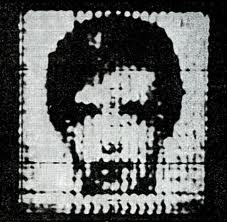
\includegraphics[height=0.75\textwidth]{images/K7PqL}
		\decoRule
    \caption[Mechanical Chair Image]{The image displayed by the mechanical chair.}
    \label{fig:chair_image}
  \end{subfigure}
  %
  \begin{subfigure}[b]{0.4\textwidth}
		\centering
    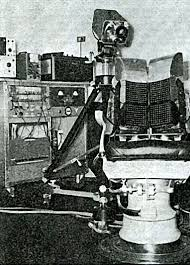
\includegraphics[height=0.75\textwidth]{images/fnJ33}
		\decoRule
    \caption[Mechanical Chair]{Brobdingnagian mechatronic device with moving attachments.}
    \label{fig:chair}
  \end{subfigure}
	\caption[Mechanical apparatus for sensory substitution]{}
\end{figure}

Moving further back into history, a Nature paper \parencite{white_vision_1969} by the same author 34 years before reported a mechatronic device which consisted of a chair that had a series of vibrating devices attached to the back, and cranks by which a camera could be moved by subjects. 400 lbs in total, the bulky device provided a similar experience, albeit with the limitations of the computing technology of its time.

Despite the experiments revealing that subjects were able to perform complicated visual processing tasks solely based on input from the chair (with only minimal training), the methods proved unusable in the industry due to a multiplicity of factors \parencite{phillips_predictors_1993}. The devices placed the user in significant discomfort, were complicated to use and relatively low-resolution, all in addition to being prohibitively expensive and limited by the technology of their time.

Since then, a number of devices \parencite{noauthor_brainport_nodate} have been released that attempt to make use of this method, but none have found mainstream commercial success \footnote{\parencite{se_perception_nodate}}.

Given the improvements in technology related to processing power, portability and hardware quality, renewed attempts are clearly needed.

\section{Claims}

This paper presents the following original contributions:

\begin{enumerate}
	\item A hardware device for haptic sensory substitution along with a short evaluation of existing hardware and software stacks, as well as designs for the construction of such a device.
	\item Multiple implementations for sensory substitution using haptic feedback, using continuous feedback processes as well as delayed-feedback spatial navigation tasks, each of which include:
		\begin{enumerate}
			\item a front-end for providing visual input to the user during the training phase, as
		 	well as useful readouts to the researcher,
			\item a transmission protocol, which maps information from the task at hand (spatial coordinates, velocity information, etc) to time-based sensor actuation signals (20$^{\circ}$ on servo 1, 35$^{\circ}$ on servo 2, etc) in real-time.
		\end{enumerate}
	\item Multiple metrics for the evaluating the performance of a sensory substitution system, as well as sample tasks that can be used to standardise and compare performance across the board for future research.
\end{enumerate}

In addition, code for displaying results in real-time, modules for managing servo overload, network latency and other factors was also written by the author.

\section{Related Work}

Some of the work that has been previously undertaken involve aiding the visually impaired in navigation and object recognition. These were helpful in identifying primary methods of communication with the brain through haptic feedback. The knowledge was used to construct early versions of a framework\footnote{In the course of this paper, the terms \textit{framework} and \textit{system} are used to describe the complete end-to-end sensory substitution module.} for providing signals to the brain, in a way that could be quickly iterated upon to find novel solutions.

\begin{figure}[th]
	\centering
  \begin{subfigure}[b]{0.4\textwidth}
		% \centering
    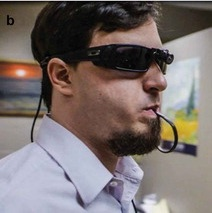
\includegraphics[height=0.75\textwidth]{images/Brainport}
		\decoRule
    \caption[BrainPort Device]{Brainport Device.}
    \label{fig:bp1}
  \end{subfigure}
  %
  \begin{subfigure}[b]{0.4\textwidth}
		% \centering
    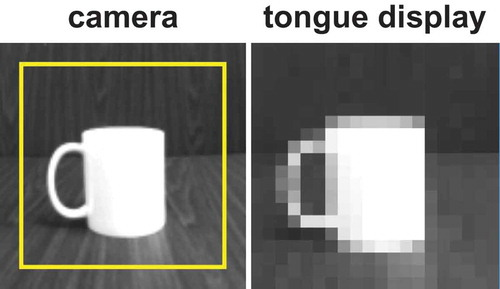
\includegraphics[height=0.75\textwidth]{images/Brainport2}
		\decoRule
    \caption[\textsc{BrainPort} images]{Captured and transmitted images from \textsc{BrainPort}.}
    \label{fig:bp2}
  \end{subfigure}
	\caption[\textsc{BrainPort} implementation]{}
\end{figure}

\textsc{BrainPort} \parencite{upson_tongue_2007} implements an industrial version of the aforementioned \parencite{bach-y-rita_seeing_nodate}. Figure~\ref{fig:bp1} shows the modifications made since the original, resulting in a smaller device that can fit on a pair of eyeglasses and requires an additional battery pack not in view.

Despite having received considerable funding and attention in the media, clinical trials of the device \parencite{nau_acquisition_2015} encountered a number of problems which then became part of the primary focii of our endeavor. Studies report the device as having "poor spatial acuity" \parencite{stronks_visual_2016}, as well as severe limitations in temporal resolution. The primary cause of these problems is attributed to the "limited bandwidth of perceived information" that the device is capable of. We aim to address these primary concerns by building a metric that can measure and improve on transmitted\footnote{In order to maintain the analogy of "signal transmission" to the brain, the verb transmit will be - unless otherwise stated explicitly or contextually - used to indicate the information being conveyed to the user from a system, usually at the exact point of the Human-Computer Interface.} effective bandwidth (something we will cover later in this section), spatial acuity, and temporal resolution.

\,

\begin{figure}[ht]
\centering
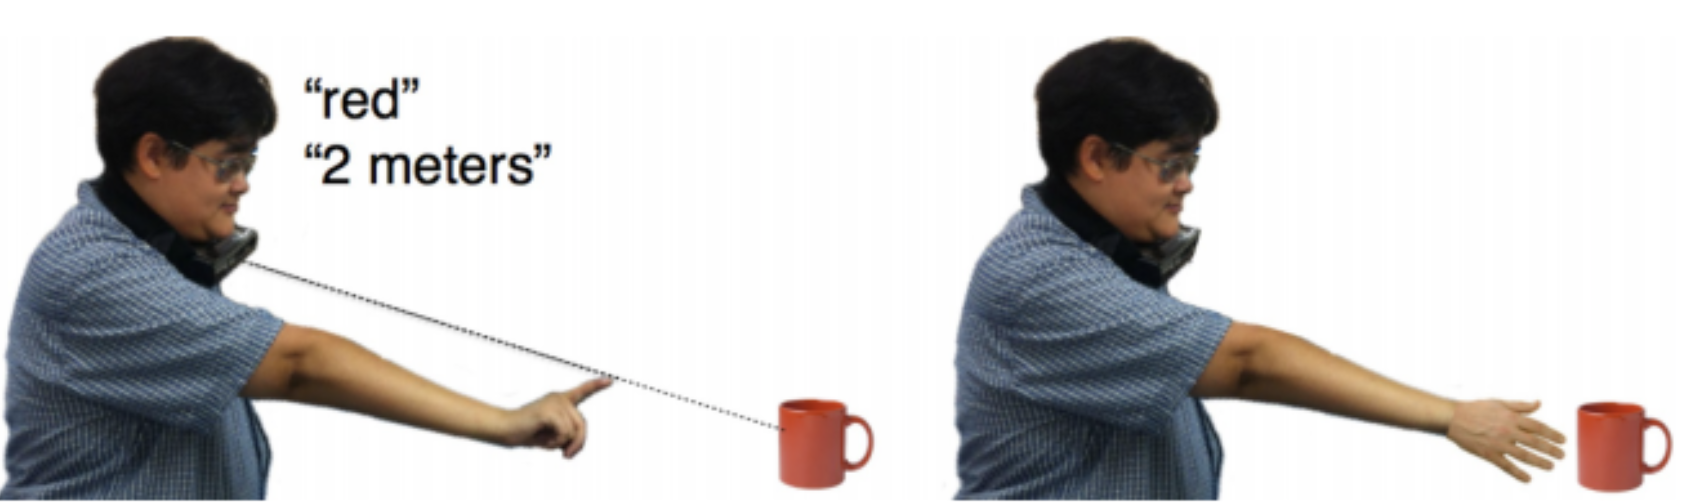
\includegraphics[width=0.7\linewidth]{images/GIST.png}
\decoRule
\caption[GIST Interface]{Demonstration of the GIST audio-spatial interface}
\label{fig:gist}
\end{figure}

Since then, the advances in processing capability and computer-vision have led to projects that make use of real-time image processing. \textsc{GIST} \citep{khambadkar_gist:_2013} is a device that provides additional information to a user as to what he is pointing at. Figure~\ref{fig:gist} demonstrates this device in operation. While initially quite promising, the device cannot be expected to work well in realistic scenarios. Due to the use of bulky external depth sensors that require non-mobile sources of power, the device is not truly portable. In addition, the authors report that scanning any object in the non-dominant side of a user causes the device to recalibrate (due to a consequent small turn of the torso). In addition, the device reports only two slow-updating channels of information. The two channels are the distance to an object and the color (presumably limited by the resolution of descriptive color words in English). One other project \parencite{akhter_smartphone-based_2011} attempts to use smartphones to create and process stereo information for depth sensing, but the project has not reached the testing stage.

\begin{figure}
\centering
\begin{minipage}{.5\textwidth}
  \centering
  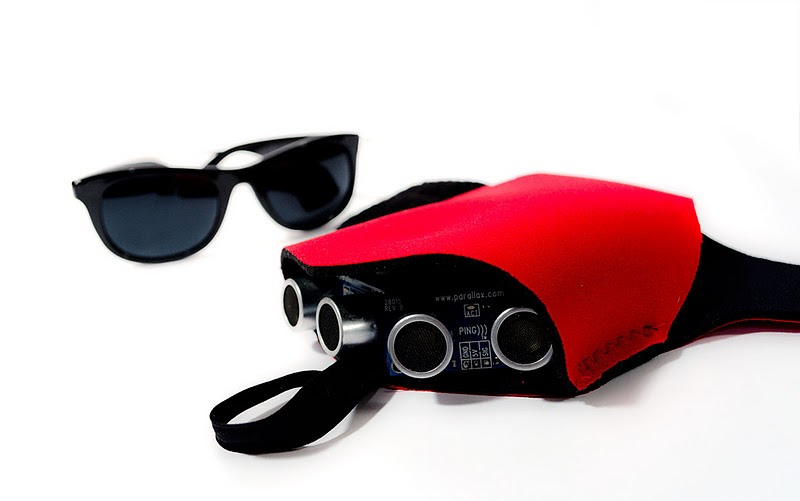
\includegraphics[width=.35\linewidth]{images/tacit}
  \captionof{figure}{Structure of TACIT.}
  \label{fig:tacit1}
\end{minipage}%
\begin{minipage}{.5\textwidth}
  \centering
  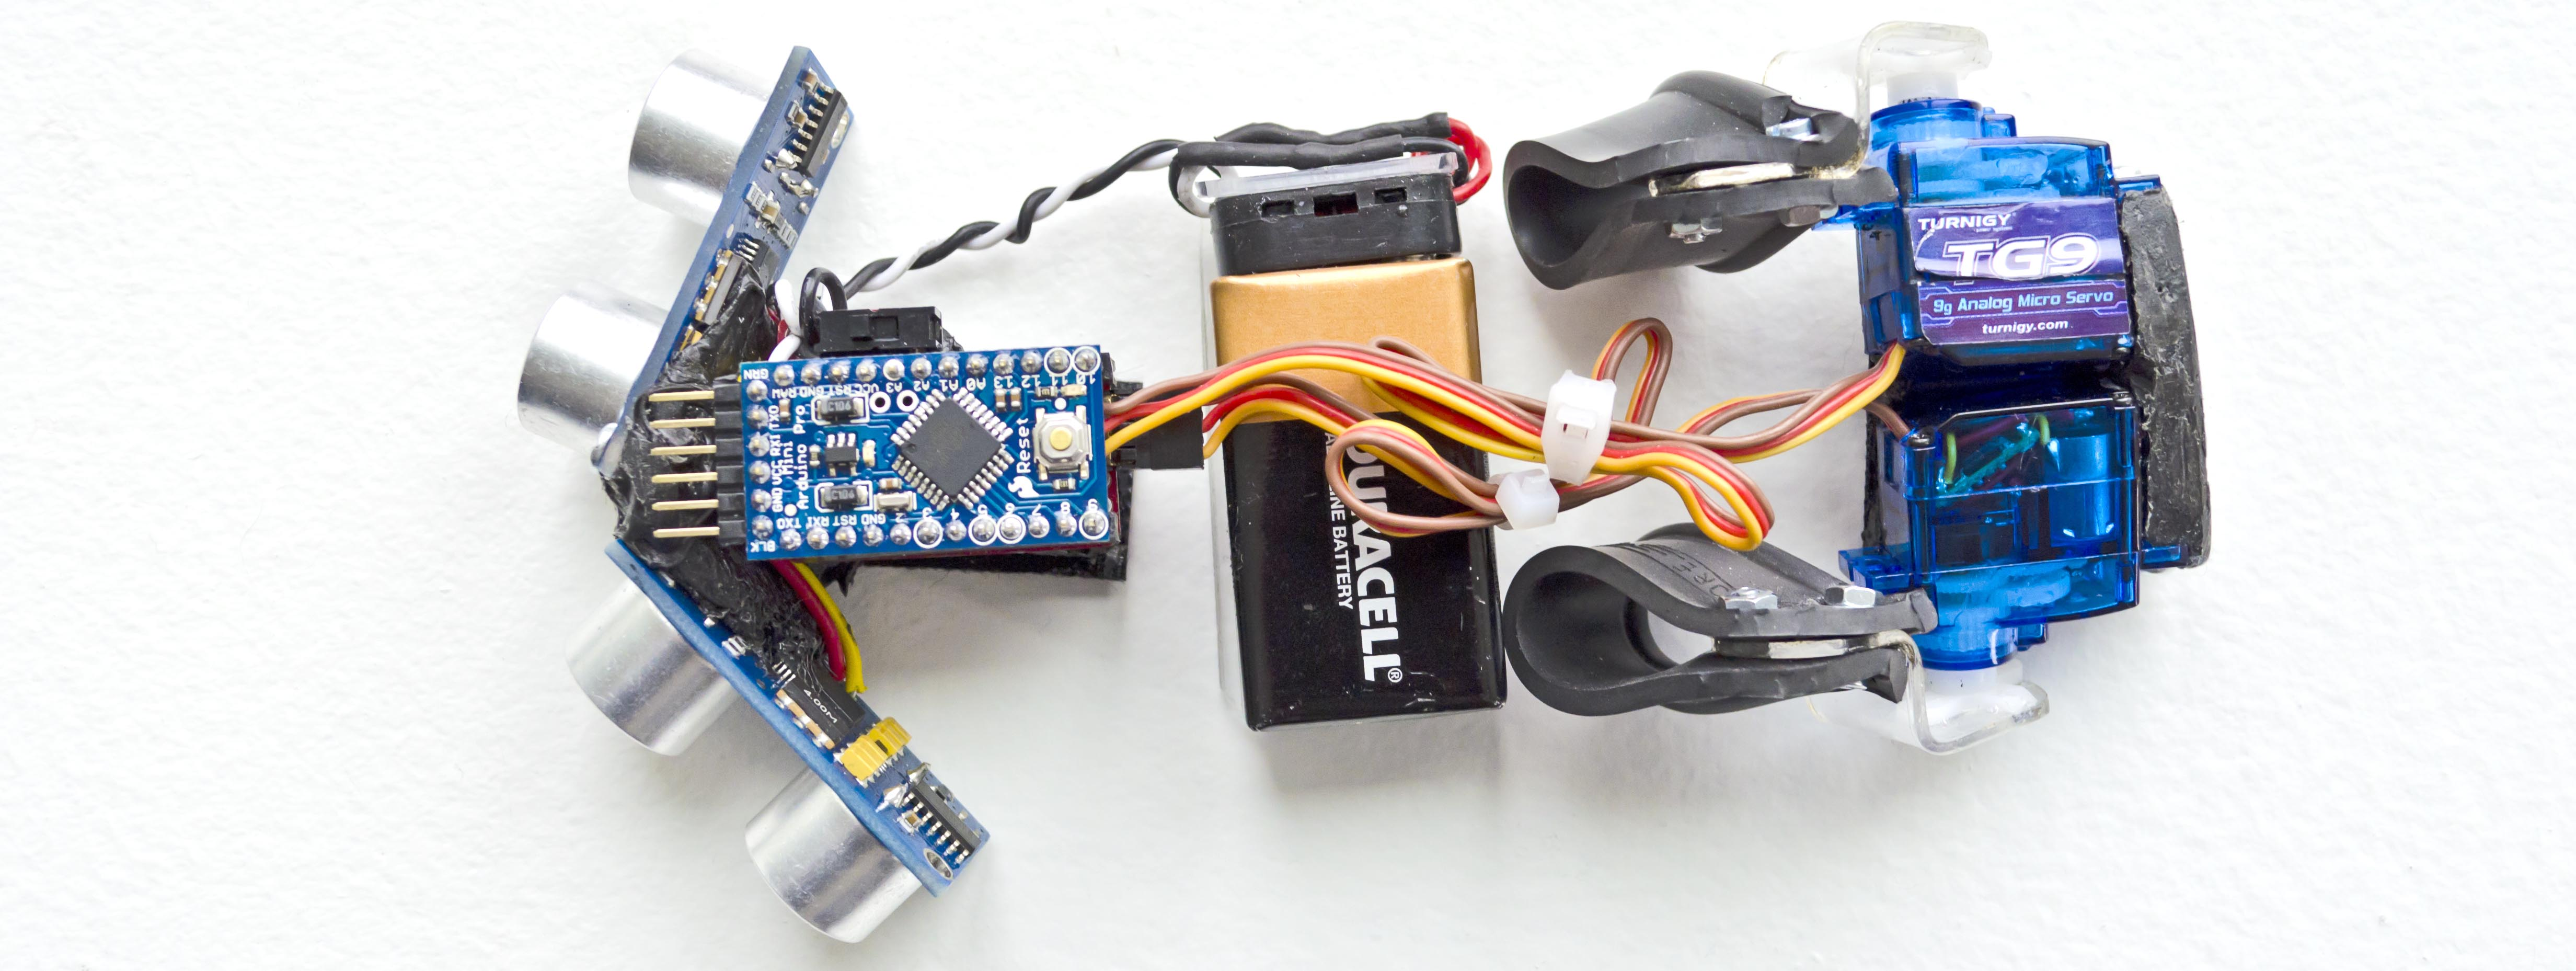
\includegraphics[width=.5\linewidth]{images/tacit2}
  \captionof{figure}[Servo arrangement]{Internal circuitry demonstrating the arrangement of servo motors.}
  \label{fig:tacit2}
\end{minipage}
\end{figure}

The project that comes closest to solving some of these problems is the Tacit Project \parencite{hoefer_meet_nodate}, which attempts to use stereo ultrasound sensors to convert distance information to haptic "squeezes" on the user's arm. Despite not containing any field tests or experiment results, my interest in the project is primarily because it aligns with the goals we have been forming from review: It is cheap, portable, relatively high bandwidth and places importance on temporal resolution and continuous signaling. Unfortunately, the lack of any experiments demotes us to reading comments and online opinions from users who \emph{do not} possess the device. In addition, Tacit is limited in temporal resolution, as it implements delays of up to 500ms between actuations, effectively being limited to a near 1 Hz frequency.
From the projects we've considered, a clear set of goals can be formulated from which to build a framework, and a number of metrics that can be used to evaluate such a system.

A well-known paper \parencite{m._fitts_information_1992} in Human Computer Interaction from 1954 outlines Fitts Law, a predictive model that can be used to calculate the time taken for a one-dimensional movement-based task from the distance moved and the size of the target. While one-dimensional movement cannot be easily extended to spatial navigation, there is merit in observing the time taken from an information theory standpoint. Below, we will also attempt to develop a set of metrics that can be used beyond the scope of this experiment to determine the theoretical maximum bandwidth of sensory substitution systems, if there exists one.

\chapter{Development}
\label{Development}

From the projects we've considered, a clear set of goals can be formulated from which to build a framework, and a number of task-based metrics that can be used to evaluate such a framework. The distinction here is that the goals concern its construction, designed to maximize the utility of the system to an end-user while the metrics are intended to be used in measuring performance with comparison in mind.

\section{Goals}

The goals of the system are as follows:

\begin{itemize}
\item \textbf{Generalizable Transmission Protocol:} One of the primary challenges of sensory substitution lies in mapping data from one realm to the sensory realm that is used to convey the information to the user. This is also a function of the human sensory infrastructure. For example, hearing operates by mapping specific wavelengths of sound waves to hair strands in the ear that convert the amplitude into intermittent electrical signals. Arguably one of the most important parts of the system, the aim of isolating the transmission protocol is to develop, compare and decide from a number of encodings for information streams encountered in the real world. An emphasis is placed on the protocol not being application specific in a way that hinders its application to similar tasks. Additional emphasis is placed on minimizing the calibration and testing required before deployment.
\item \textbf{Continuous Signaling:} Another conspicuously lacking element in past work is the discrete nature of the feedback provided. Systems we have looked at so far continuously snapshot the environmental signals meant to be conveyed, reduce them over a time window to a lower resolution counterpart and then transmit this to the user. Studies \parencite{kristjansson_designing_nodate} regarding the effectiveness of sensory substitution devices indicate that "spatiotemporal continuity" is significant in maintaining immersion and shortening the training and acclimatization period. Based on this, the framework prioritizes the transmission of continuous signals. Measuring and increasing the frequency (in addition to the bandwidth metrics stated above) of transmitted information is also of value.
\item \textbf{Effective Bandwidth:} While measurement of effective bandwidth is only possible in a task-based environment (after implementation), it is a priority in design to ensure that the no part of the system is the bottleneck in conveying this information. This will involve making sure that network latency (when involved), as well as the hardware limitations of the device are understood and accounted for.
\item \textbf{Spatial Acuity: }The project will primarily focus on spatial navigation and other related objectives for the experiments, as implementing them on a realtime system will also satisfy the temporal acuity goal. The objective is to convey information regarding full 3-dimensional\footnote{It is worth noting that the related works we have considered resort to slicing 3-dimensional space to present a 2-dimensional version to the user. It is an interesting question if this approaches a fundamental limit.} space and object recognition with the intent of performing tasks.
\item \textbf{Portability:} The rise of personal mobile devices presents an opportunity that had been closed to most previous studies. Attempting to make the implementation less expensive and more mobile and self-sufficient will be a priority. This means reducing the number of separate modules, reliance on experimentally determined conditions and power consumption just to name a few attributes.
\end{itemize}

The purpose of these goals is to serve as reasonable guidelines on which to evaluate the results derived, as well as a possible scaffold on which future extensions can be developed.

\section{Components}
\label{Components}

In the interest of modularization, the framework can be subdivided into the following general components, each with as close as possible to a distinct set of constraints, technical stacks and parameters for optimization:

\begin{enumerate}
\item \textbf{Transmission Interface:} The (primarily) hardware component that transmits (via haptic feedback in our case) already encoded information to the user. The optimizations here are towards making the system as responsive as possible, minimizing latency, as well as deciding the best components and control circuitry to improve the experience. As we will see later, even a choice of fabric for the instrument case or the type of soldering involved can have a major impact.
\item \textbf{Signal Encoder:} Despite the hardware-sounding name, this is primarily software-based, and handles the encoding of incoming sensor streams (with minor prior correction) to outgoing activation signals. From experiments, the location of this module is important - placing it as close to downstream\footnote{Terminology: Upstream is closest to the front-end while downstream is closest to the user.} as possible leads to lower latency, however there is a delicate balance to be struck. Devices tend to have more processing power as you move upstream, promising significant speedups that can offset the loss from distance.
\item \textbf{Application:} This is the module that handles most tasks needed to ensure that the entire system is operational, including a networking module, display management, device enumeration and asynchronous processing, logging, etc.
\item \textbf{World Interface:} The World Interface handles all aspects of the task being performed by the user. This may range from simulating a Virtual Reality environment to computer-vision based mapping and tracking of spaces for an Augmented Reality task. Task completion is also measured and reported from this module.
\end{enumerate}

\chapter{Experiment}
\label{Experiment}

Now we can move to the tasks, as well as the metrics associated with them. The tasks, metrics and results are divided into Phases 1 and 2, where Phase 1 explores continuous-feedback based navigation in two dimensions. Phase 2 then builds on the work in Phase 1 to explore delayed-feedback based spatial navigation in three dimensions using a Fitts' test. The metrics are explored here, but the results are grouped in the results section afterwards.

\section{Phase 1: Sightless Racing}

In Phase 1, the virtual space of a car and race track were mapped to a haptic device. The primary aim of the experiments were to see if users with some training could intuitively drive the car around the track, dodging obstacles and following the road.

With this in mind, the tech stack used is below in keeping with the module separation outlined in Section~\ref{Components}:

\begin{enumerate}
\item \textbf{Transmission Interface:} The Transmission interface consists of servos that are rated at 1.6 kg-cm in torque, arranged on a flexible plastic film wrapped around the user's arm. The servos are outfitted with 3 cm arms that rotate down to push lightly into the user's skin, connected to a Raspberry Pi Model B, running a python server which communicates with the front-end. Figure~\ref{fig:device1} shows the device as it is fitted to the user's arm.

\,

\begin{figure}[ht]
\centering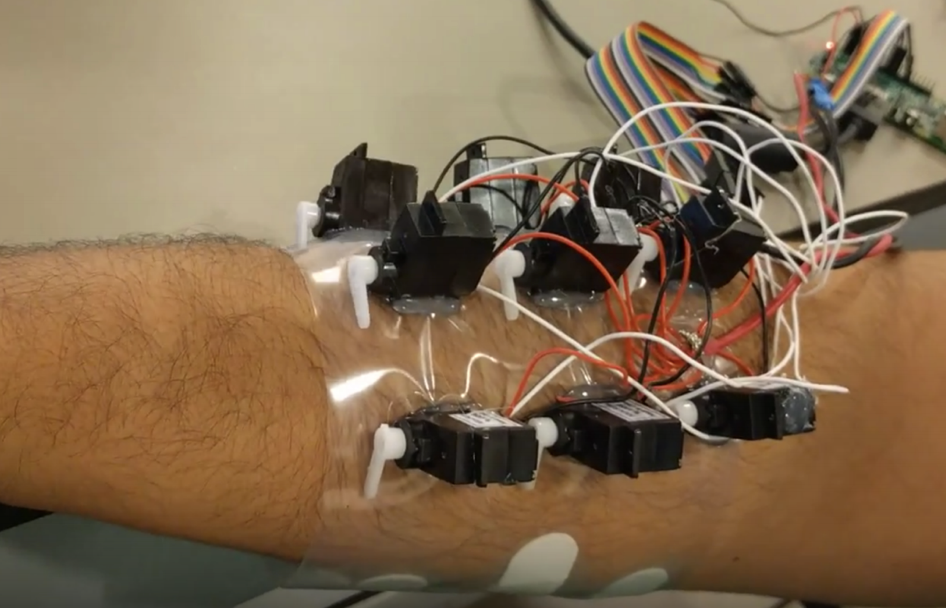
\includegraphics[width=0.7\linewidth]{images/v1device.png}
\caption[P1 Device]{Phase 1 Transmission Interface on a rather large arm.}
\decoRule
\label{fig:device1}
\end{figure}

The basic material used for construction was determined after much trial and error. Optimizing for maximum sensitivity, the first configuration enabled the arms of the servos to directly make contact with the skin. While this did achieve the intended purpose, users were overstimulated and described sensations of "sensory overload" and "uncomfortable stretching and pulling". Fabric was the second option, but was overtly effective in dampening sensitivity and preventing users from distinguishing the servos, as well as adding noise due to the texture rubbing against the skin. In addition, fabric proved to quite unhygienic due to being permeable and receptive to sweat and grime, which made it unsuitable for continued use (especially with multiple participants). The ideal option proved to be the ESD-safe plastic bag that the servos arrived in - comfortable without being sharp around creases and stretch-proof, it had the added advantage of not carrying odors.

\item \textbf{Signal Encoder:} The Transmission Interface makes use of a 3x3 grid of servos, placed in a square on the user's arm (Figure~\ref{fig:device2}). Preliminary (with one or two participants) pilot testing helped eliminate configurations such as a strip around the arm, crowded circle placement, and lengthwise across the arm due to lack of sensitity and general discomfort. The final wide configuration also provided the advantage of being adaptable to other locations on the body, and easier to map in software.

\,
\begin{figure}[ht]
\centering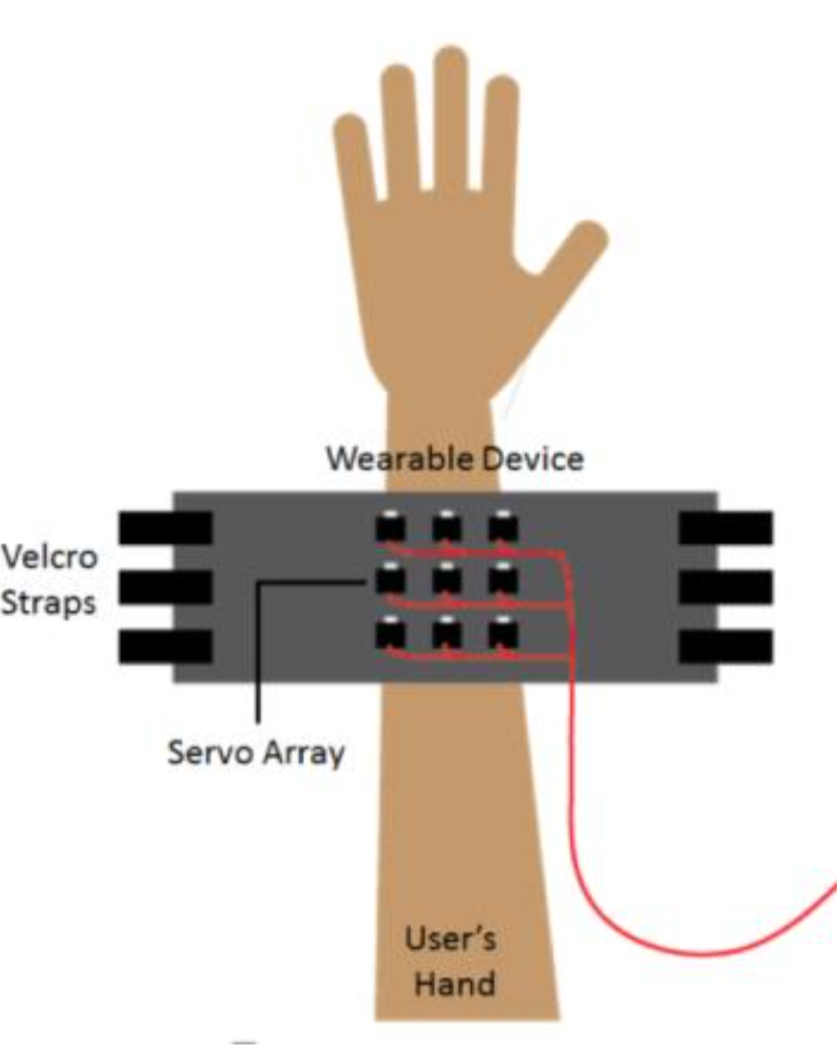
\includegraphics[width=0.4\linewidth]{images/v1device2.png}
\decoRule
\caption[Servo configuration]{Servo configuration.}
\label{fig:device2}
\end{figure}

The configuration contributed to the activation patterns in the Signal Encoder. Pilot testing revealed that the four corners were the most identifiable, and that the servos in between contributed to immersion.
The information received was consolidated into four analog time streams, which was subsequently converted to discrete values of 16-bit resolution, which was then frequency modulated \parencite{noauthor_frequency_2017} and amplified to produce the activation signals for the corner servos. Figure~\ref{fig:plot1} shows how the activation signals are combined. For the servos in between the corners, a discrete signal was generated for them by alternating between their neighbors using a base frequency and likewise coded in frequency with a fixed amplitude.

\,

\begin{figure}[h]
\centering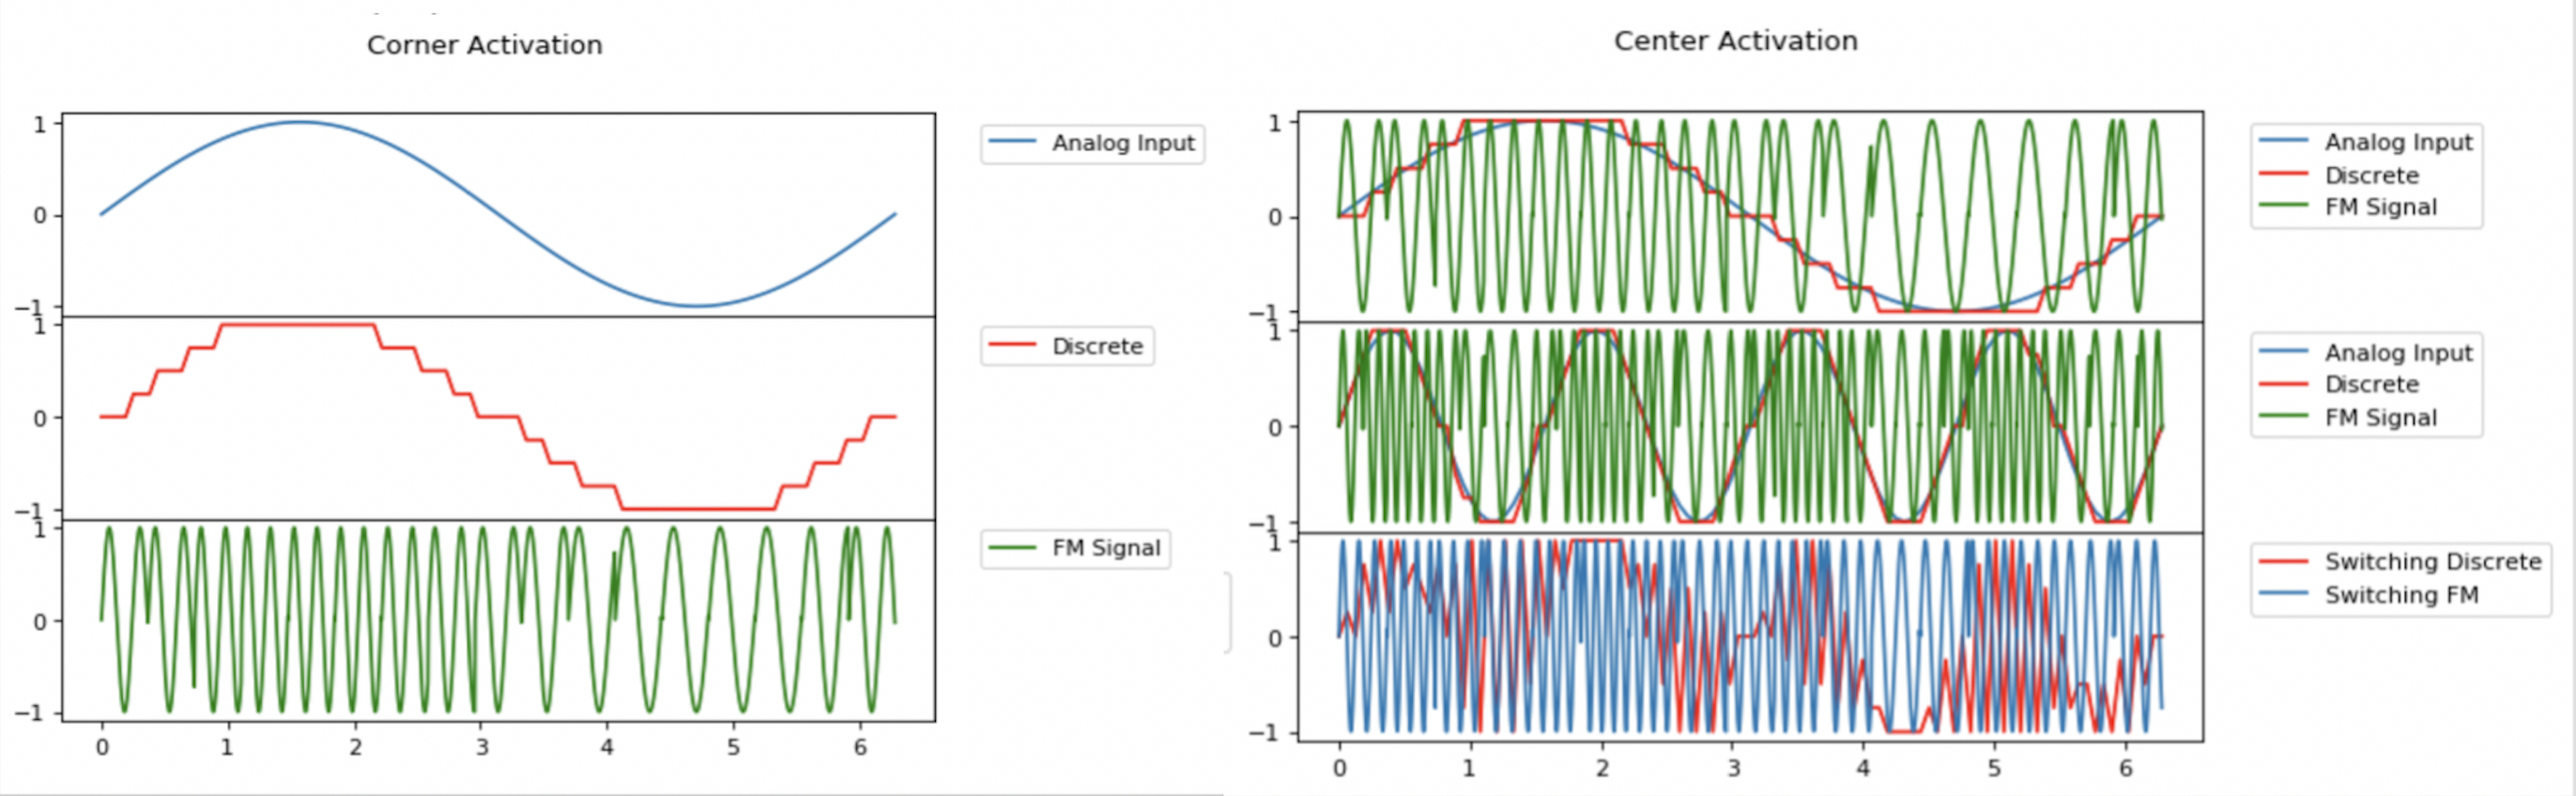
\includegraphics[width=1.0\linewidth]{images/plot.png}
\caption[FM switching visualization]{Visualization of switching FM implemented in activation.}
\decoRule
\label{fig:plot1}
\end{figure}

This particular signal pattern proved most effective in shortening training times and providing immersion and the strongest sensory substitution as reported by the early participants.

\item \textbf{Application:} For Phase 1, the application was developed to optimize for fastest turnaround time in code sprints, using python and Javascript to make the process easier. A webserver written in Javascript listens asynchronously for signal broadcasts from the World Interface, and the upstream packet transmission is managed by a python webserver working in conjunction with the World Interface application.

\,

\begin{figure}[h]
\centering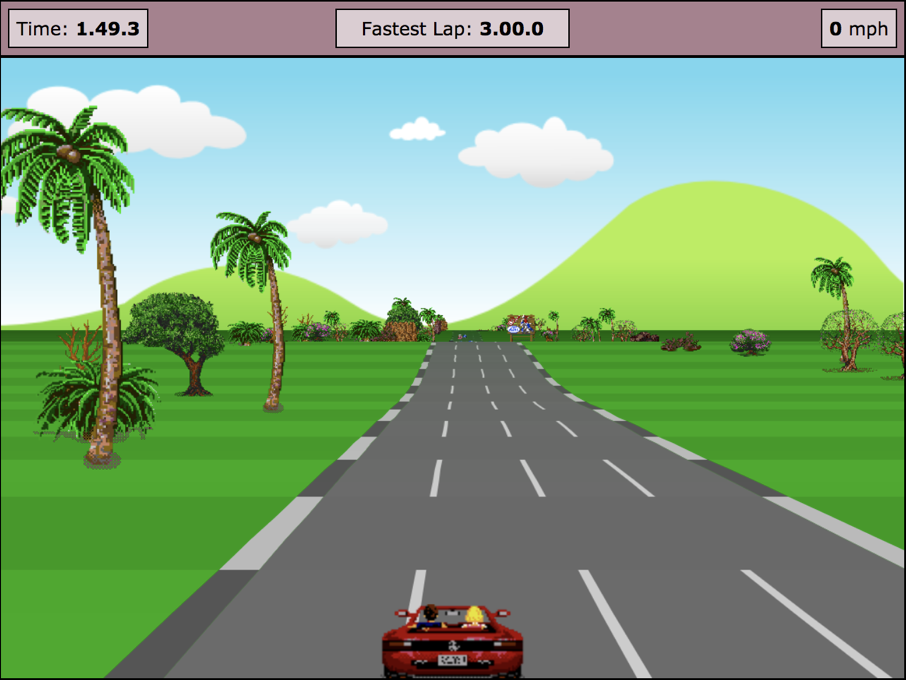
\includegraphics[width=0.5\linewidth]{images/race.png}
\caption{Implementation of the World Interface.}
\label{fig:outrun}
\end{figure}

\item \textbf{World Interface:} The primary purpose of Phase 1 was to find the best possible signal encoding for real-time time-variant data. The users were presented with a familiar gaming interface resembling OutRun \parencite{noauthor_out_2017} (Figure~\ref{fig:outrun}, which made the initial introduction easier. The World Interface application responded to keyboard controls, and produced the following values as a continuous multi-dimensional vector: the current position of the car relative to the center of the road, the current position of the car relative to the road on current trajectory after t+4.0 seconds, and the positional information of obstacles.

\end{enumerate}

\,

\begin{figure}[h]
\centering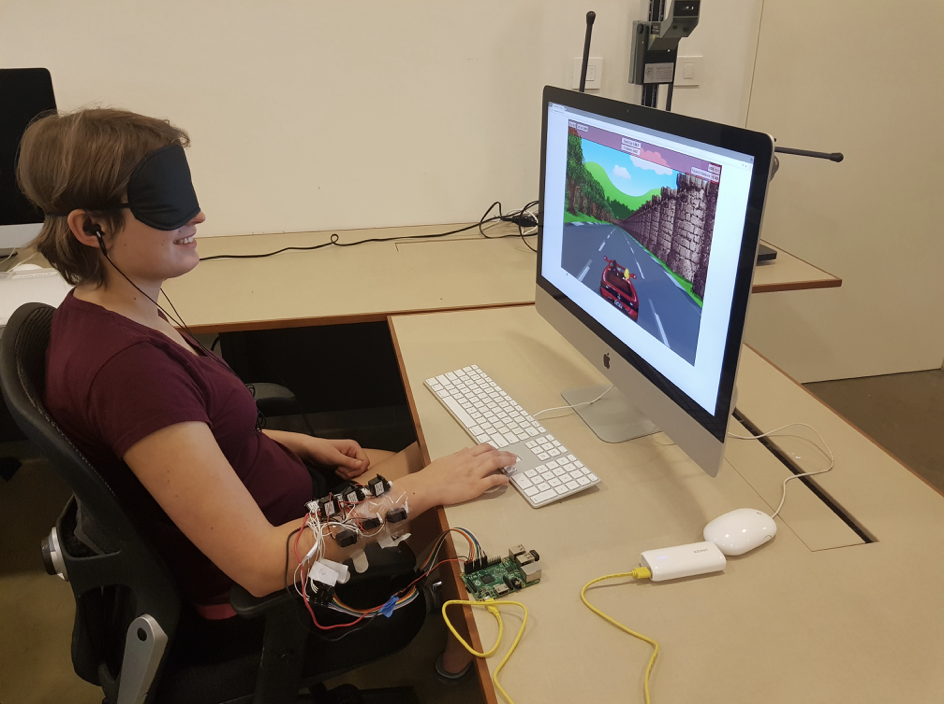
\includegraphics[width=0.5\linewidth]{images/gameplay.png}
\decoRule
\caption[P1 experiment]{Phase 1 training setup.}
\label{fig:play}
\end{figure}

The experimental setup involved a training stage and a testing stage. The training stage involved asking the participants to play the game while wearing the device for a fixed period of time (set to 10 minutes for standardisation) without being blindfolded.

Following this, the testing stage had the participants blindfolded and playing the game solely using input from the haptic device.

Due to time and resource limitations, a formal experiment for Phase 1 was not performed. The device was tested at a hackathon on subjects of ages 6--65, and the general responses have confirmed it as an effective method of sensory substitution. With ten minutes of training (and no instruction as to the function of the device), all participants were able to play the game without crashing once out of every three laps on a procedurally generated randomized track. In addition, when encountering an obstacle or a turn in the road, all participants were able to reflexively\footnote{Interesting feature of note that differentiated other encodings was the report from users that they were 'remembering' the meaning of a signal as opposed to 'feeling' the result of a signal. My intuition is that the latter is a sign of the brain using non-conscious processing to understand the new input. Participants performed better across all categories when they reported that they were 'feeling' instead of 'remembering' (the terms borrowed from participants' recounting the experience).} judge the correct rate of turn and direction without hesitation\footnote{Younger participants were able to perform similarly as older participants with significantly less training time. This correlates with literature \parencite{kolb_brain_2011} in that age is negatively correlated with neuroplasticity.}.

\section{Phase 2: Virtual Reality Fitts Test}

Phase 2 has the participants perform a Fitts test (a pointing task that measures accuracy in a standardised way) in a Virtual Reality environment, with and without the aid of sight.
Shown in Figure\todo{Take and add a figure showing experiment setup here}, the participants follow the training-testing structure of Phase 1, where they point and click at various targets in the virtual world.

Iteratively improving on the results and design of Phase 1, Phase 2 is a more complex task in a noisier environment. For one, Phase 1 operated on continuous-feedback. The participants were continuously made aware of success and failure in relation to the task, while Phase 2 provides delayed-feedback, where the completion of a task has a much more time-dilated response. In addition, moving from two dimensions (two vectors) of critical information to three adds the potential for noise and sensory overload. With this in mind, let's consider the modular design where it deviates from Phase 1:

\begin{enumerate}
	\item \textbf{World Interface: } As Phase 2 is built on top of Virtual Reality, the World Interface proved to be one of the most complex modules in terms of design and implementation. There are a number of offerings on the market for Virtual Reality, but spatial localisation is not well implemented. Tracking an object with certainty across a 3d space is an open problem in computer vision, and acceptable solutions with low latency have only recently become available on the consumer market. The options considered included implementing SLAM \parencite{noauthor_simultaneous_2017} a resource intensive algorithm to map indoor spaces using a single camera, and the two competing Virtual Reality products on the market that offer this functionality, the HTC Vive and the Oculus Rift. The Oculus Rift was chosen for the following reasons: One, the Rift offered easily extensible tracking algorithms in the form of HTC's Lighthouse technology\footnote{An interesting video capturing the operation of the Vive's lighthouses is at \href{https://www.youtube.com/watch?v=5yuUZV7cgd8}{https://www.youtube.com/watch?v=5yuUZV7cgd8}} \parencite{niehorster_accuracy_2017}, which promised to aid future research. Two, HTC Software was closely compatible with Steam VR and Unity, which enabled faster development and turnaround times. Finally, SLAM was abandoned as it lacked a robust implementation and would require coding work equivalent in time to another capstone to implement. Some open implementations \parencite{yan_contribute_2017}
	\parencite{aivijay_lsd_slam_noros_2017} for SLAM exist, but none that can function within the constraints of a mobile device.

	The World Interface (Figure~\ref{fig:vrfittss}) contains three primary parts. The first is a Fitts Test board, which contains targets that need to be selected in a randomized order. The second is a controller that virtually represents a physical object held by the participant, and the third is a virtual pointer being extruded at the same angle as the controller. The participants can click the controller via a provided button, and are asked to select the targets as instructed through color (for sight) and the haptic device. Red represents the next target, yellow for any selected target, and green when the right target has been selected.

	\begin{figure}[h]
		\centering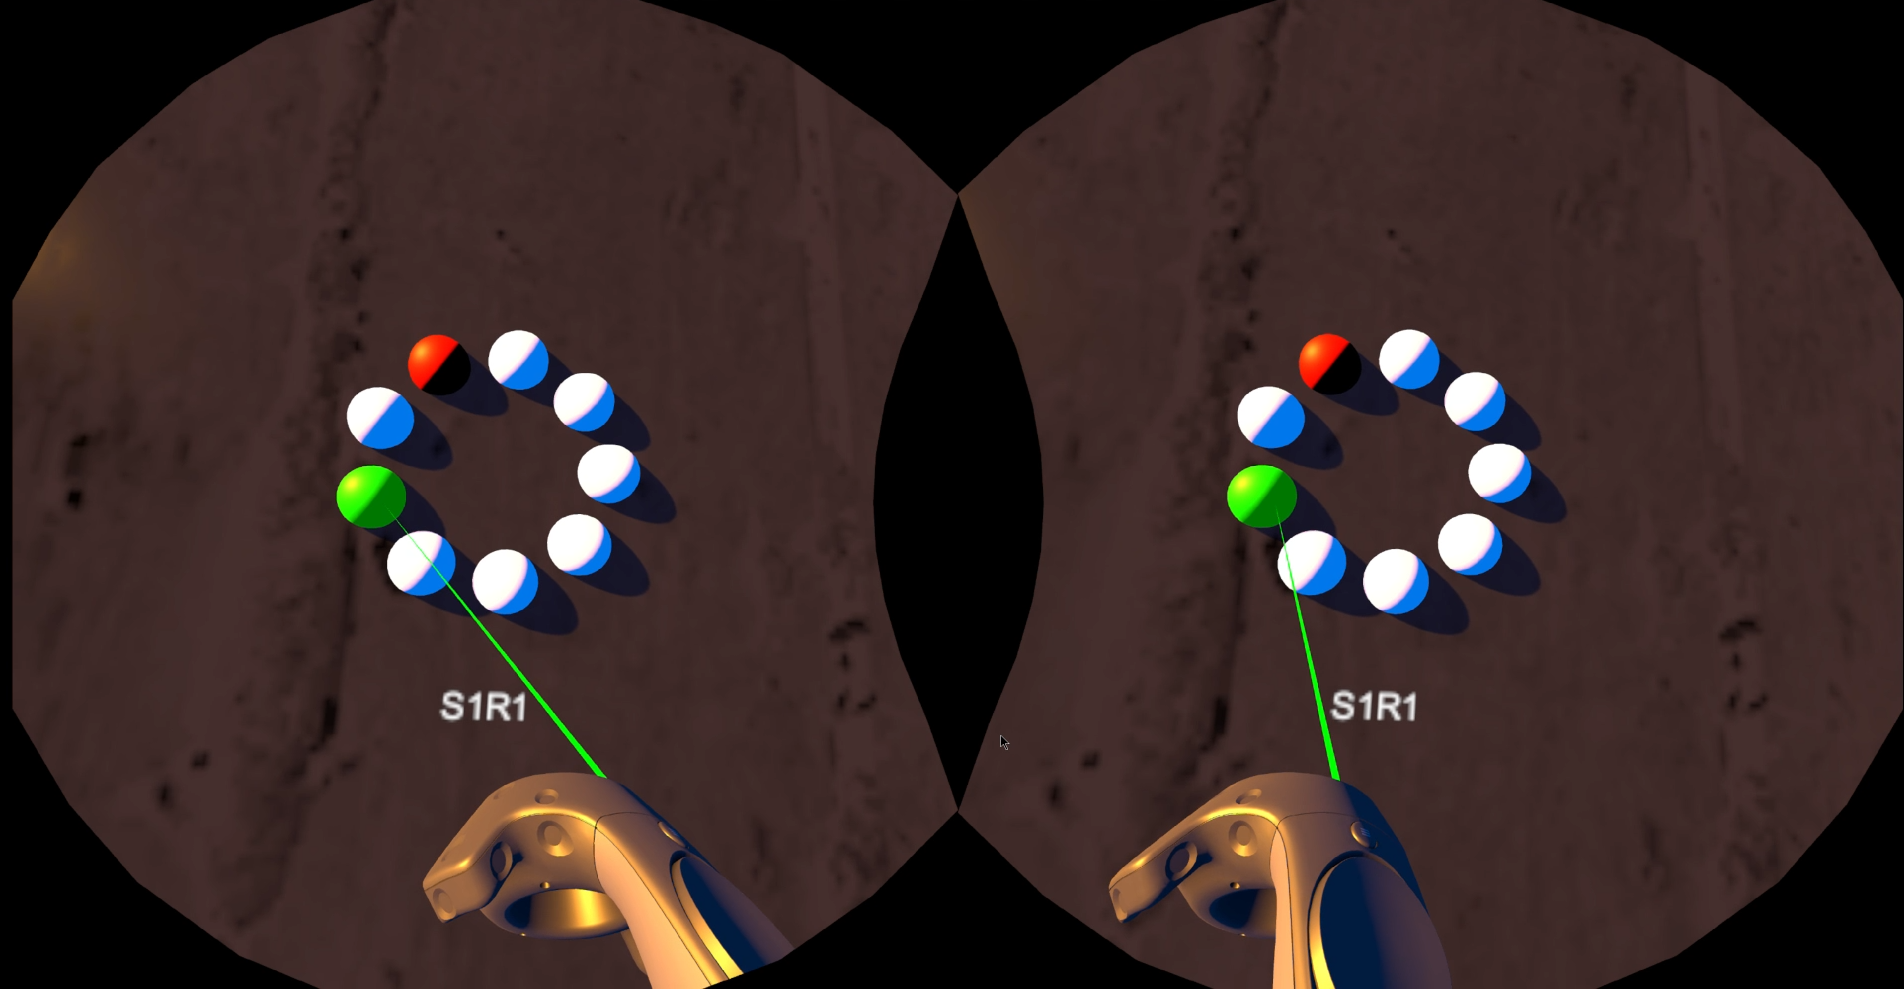
\includegraphics[width=1\linewidth]{images/vrfittsscreenshot.png}
		\decoRule
		\caption[Virtual Reality Setup]{Virtual Reality Setup for Fitts Task.}
		\label{fig:vrfittss}
	\end{figure}

	\item \textbf{Application: } The application, due to restraints imposed by the introduction of VR, was developed in C\# on the server side. The same software was used on the client side as Phase 1, with some modifications.


	\item \textbf{Signal Encoder:} The first consideration in the design of the Signal Encoder involved the mapping of spatial orientation in regards to the controller. A number of options underwent preliminary pilot testing, which included a cartesian set of vectors in 3D space, polar coordinates encoding the angle and distance to a target, and other more convoluted sets of representations. The testing revealed the most effective mapping to be a set of cartesian vectors adjusted to the user's orientation, such that the controllers' left, right, up and down were the same as the participants'. Performance was also improved when these vectors were inverted to provide adjustment information rather than absolute information (eg. 'go left to find the target' as opposed to 'you are right of the target' in terms of an instruction). For additional information, a new binary vector was added that switched to \textbf{1} for half a second when the pointer encountered the correct target to measure the effects.

	\begin{figure}[h]
		\centering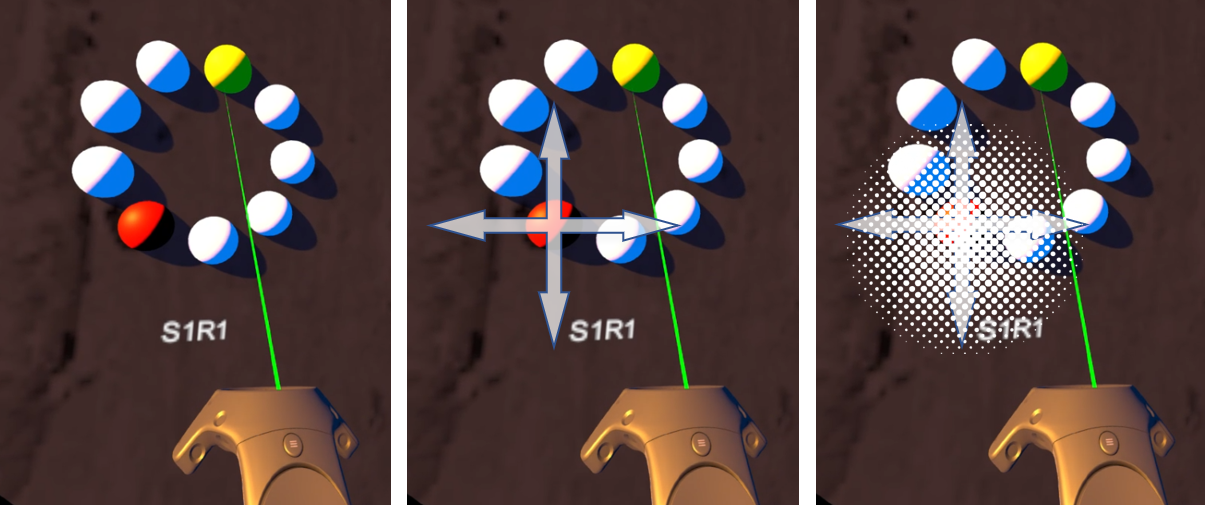
\includegraphics[width=1\linewidth]{images/fittscoords.png}
		\decoRule
		\caption[Cartesian Vectors in VR]{Overlay representing of cartesian vector magnitude and origin.}
		\label{fig:fittscoords}
	\end{figure}

	Figure~\ref{fig:fittscoords} shows a representation of the magnitude and origin positioning of the vectors conveyed through the haptic interface.
\end{enumerate}

Complete with the design, we can now move to the results.

\chapter{Results}
\label{Results}

\subsection{Experimental Apparatus}

The haptic device mentioned in detail above was made of a Raspberry Pi Model B\footnote{1.2 Ghz Quad-core ARMv8 CPU, 1 GB RAM, 40 GPIO Pins (with nine pins operating in software PWM mode). The Raspberry Pi was running the Wheezy distribution of Raspbian OS from a 16 GB micro SD card.}, which was used to drive the nine servos\footnote{Rated for torque: 0.117 Nm at 4.4V, speed: 0.15 sec/$\circ$, single-top ball bearing nylon gear servo. Part No. A0090} as part of the haptic device at 3.3V. The Rasberry Pi was run in headless mode, connected via SSH to a BASH terminal for logging. The front-end computer was a custom built desktop\footnote{Intel Core i7-6700K CPU @ 4.00 Ghz, 16 GB RAM, 64-bit Windows 10 Professional with an NVIDIA GeForce GTC 980 Ti} connected to a Sharp PN-K321 4K (3840x2160) 32" monitor with a Logi Master MX mouse and a Logi CRAFT keyboard. All trials were performed in an isolated room at Yale-NUS, away from distractions.

\begin{figure}[h]
	\centering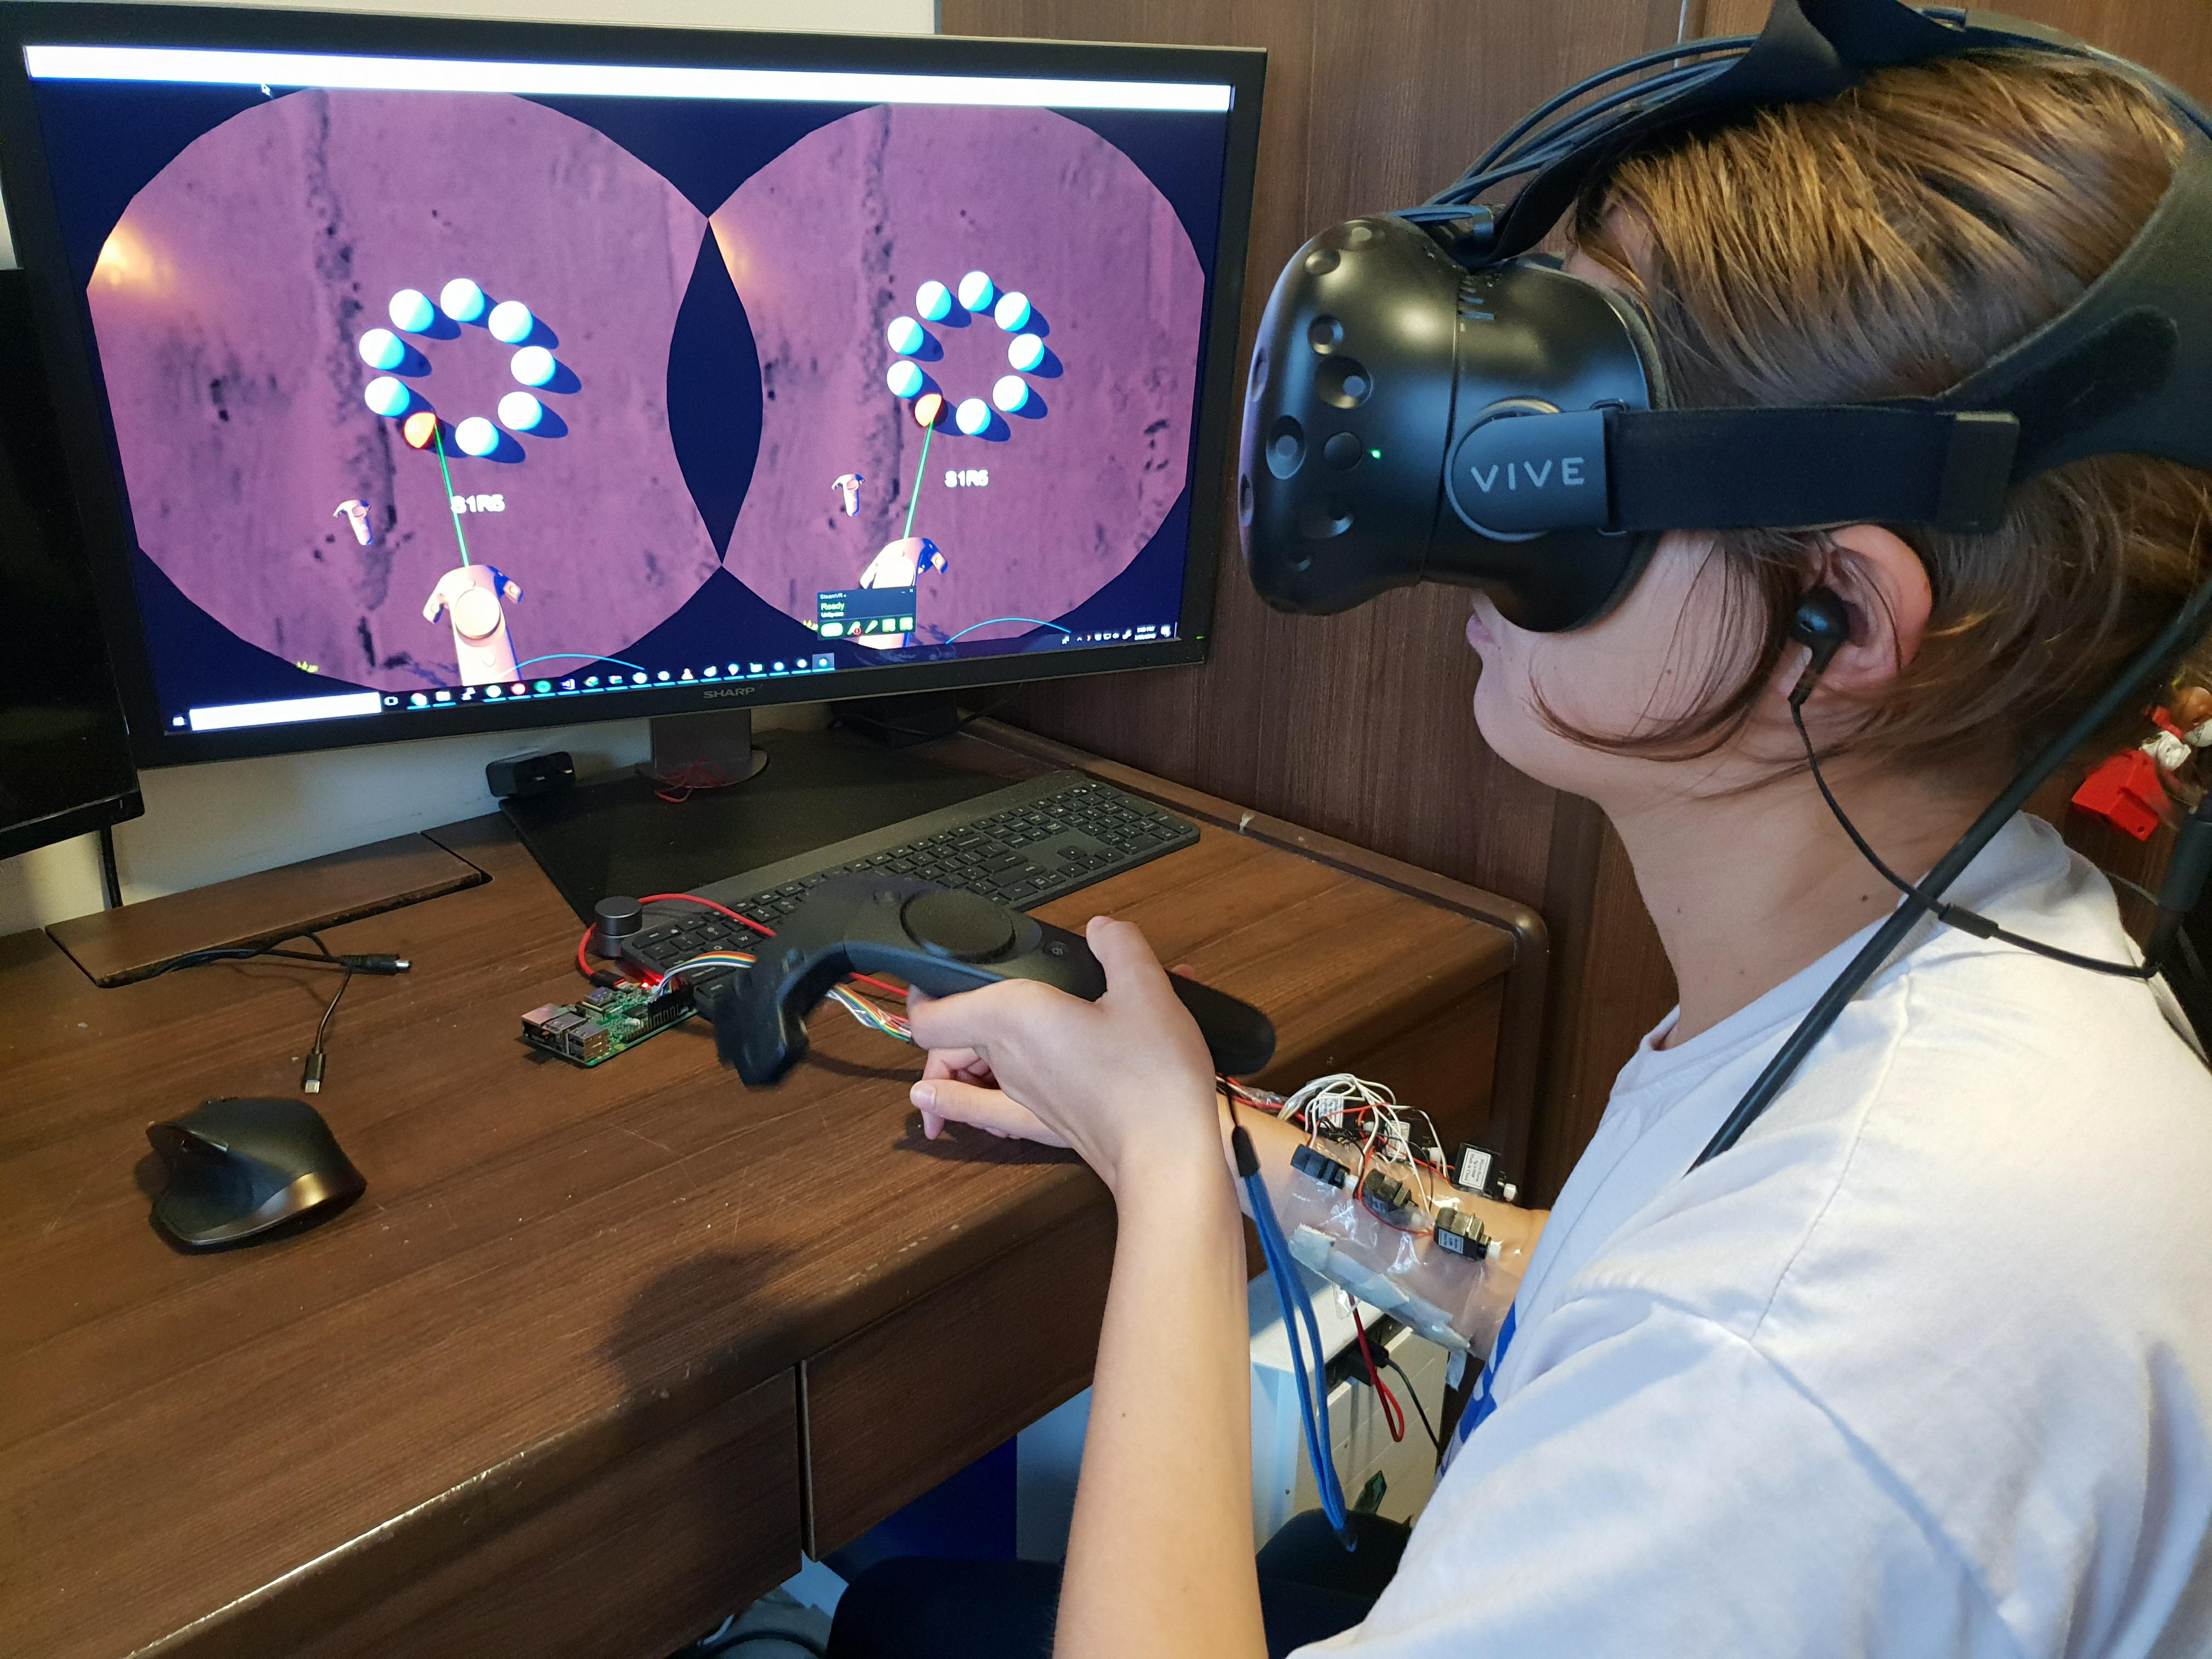
\includegraphics[width=1\linewidth]{images/experimentsetup.jpg}
	\decoRule
	\caption[Experiment Setup]{Experiment Setup showing participant.}
	\label{fig:experimentsetup}
\end{figure}

Figure~\ref{fig:experimentsetup} shows the experiment configuration.

For Phase 2, the HTC Vive Virtual Reality headset was used in stock configuration. In addition, the multi-core CPU on the Raspberry Pi was used in Phase 2 for multi-threaded operation, which permitted a web server to receive signals, and another thread on the same server to actuate the servos. Raspbian is not a realtime OS, so some timing variation is expected. However, for the timings in question it should not be noticeable.

\section{Experimental Design}

Pilot testing for Phase 1 was performed at a hackathon, with 7 participants (2 female, 5 male) after which the data was aggregated and anonymized. Each participant was given five minutes of training and five minutes of testing (blind) time, and the participants were between 18 to 25 years of age.

8 participants (2 female, 6 male, 1 left-handed, 7 right-handed) were selected for testing Phase 2 of the prototype. All participants were between 18 to 25 years of age. Informed consent was obtained from all participants beforehand, and the experiment lasted 45-minutes on average.

\section{Phase 1}

Phase 1 results were collected primarily in a single dimension: error. The error was measured as the l2norm distance of the car from the centre of the road and timestamped. This data was then interspersed for purposes of anonymity, and is presented in Figure~\ref{fig:p1error}.

\begin{figure}[h]
	\centering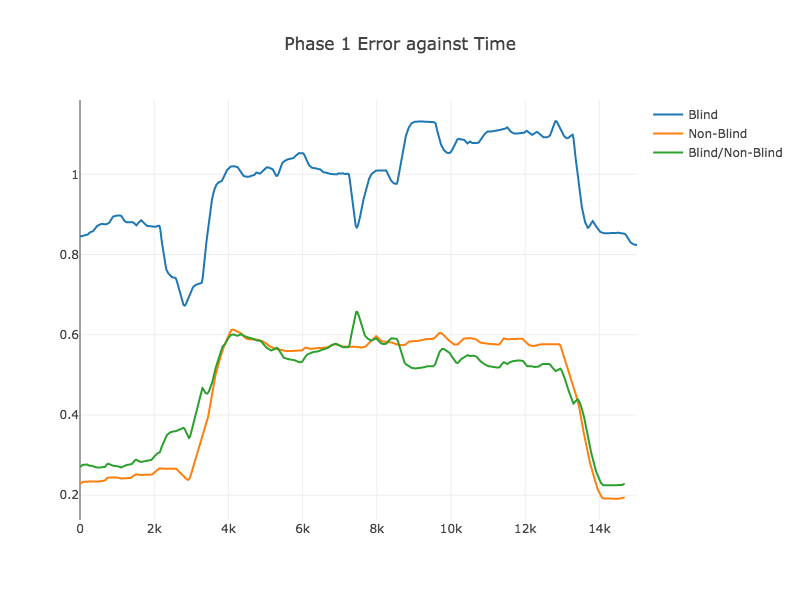
\includegraphics[width=1\linewidth]{images/p1error}
	\decoRule
	\caption[Phase 1 Error]{Phase 1 Error Graph.}
	\label{fig:p1error}
\end{figure}

From the graph, we can see that the error when playing blind is still within the same order of magnitude as the error with sight. Participants were able to correctly steer the vehicle and complete multiple laps of the track without visual aid. Correcting for the procedurally generated track with easier and tougher sections, we can see that graphing blind error over non-blind shows a training effect where the error decreases over time\footnote{Note that this is preliminary testing and needs to be confirmed through further experiments.}.

\section{Phase 2}

In Phase 2, the Fitts' Test is used because it is currently a standard in measuring human-computer interfaces. Fitts' Law is useful in our case, but it is only peripherally relevant to the scope of this paper. Measuring the information-theoretic maximum of a sensory substitution model is something that deserves an exploration on itself, and is therefore left to future research. The Fitts' Test however, provides data that can be used by other researchers to compare our data and to compile a growing dataset. It therefore stands to reason that our primary measurements be the same as those in a Fitts' Test. The primary measurements that are common in this modality \parencite{mackenzie_extending_1992} \parencite{chun_evaluating_2004} are the time taken to reach a target, and the distance from the center of the target when a successful click is made (also called error).

The Fitts' Test was performed in four sessions comprising of five blocks, each block representing one complete circle where all targets were selected. Of the five blocks, information from the first block was discarded and marked as training. Among the four sessions, two independent variables were chosen and varied across the sessions. The two variables were whether the participant had sight (blind vs non-blind), and whether an alert-tone (as described above) was given (alert vs non-alert).

In addition, the time taken to reach an individual target is also affected by the distance between the two targets. This was corrected by dividing the total time taken for each target by the distance between the previous target and the intended target.

\begin{figure}[h]
	\centering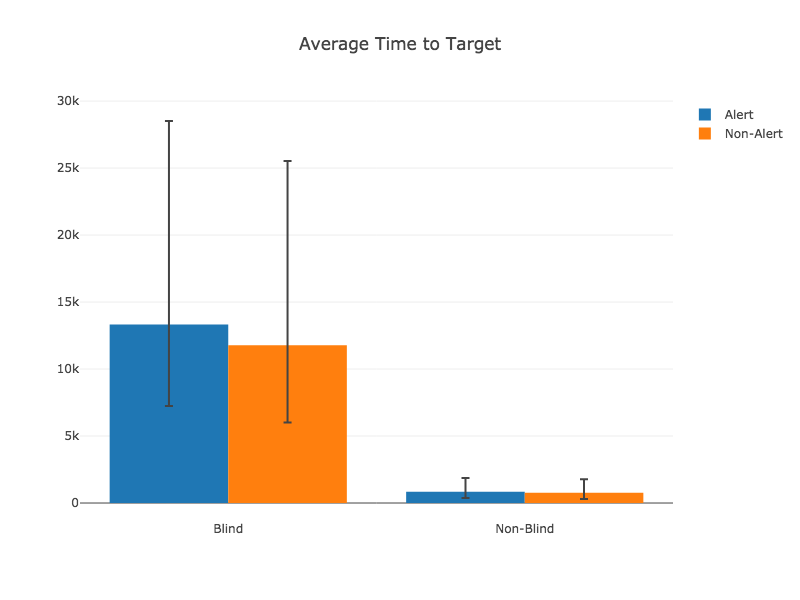
\includegraphics[width=1\linewidth]{images/timetotarget}
	\decoRule
	\caption[Phase 2 Time to Target]{Average time to target (adjusted for distance).}
	\label{fig:p2time}
\end{figure}

Figure~\ref{fig:p2time} shows how the average time to target, corrected for distance, varies across the two parameters. Changing the blind component affects the average by more than two orders of magnitude, which is very different from the results we observed in Phase 1. This is presumably due to the added noise and variation involved in the system, along with the delayed-feedback mechanism at play.

We can also see that there is a lot more variation in the blind trials, and this was confirmed by the researcher as the participants often vascillated heavily in deciding which direction they needed to move in. What is interesting is that providing an alert notification increases the amount of time taken to hit a target. While counter-intuitive, in practice it was observed (and reported by participants) that the alert notification worked counter to the participant training him/herself to learn the other signals. What was even more surprising was that this remained true even when the participants could see the targets in front of them. The alert tone proved to be a distraction that lengthened training times and possibly prevented the participants from `feeling` the signals being conveyed.

ANOVA confirms this intuition as we can see in Table~\ref{tab:p2timinganova}. There is a strong effect on blind vs non-blind on the time taken to hit a target ($p < 9.6 \times 10^{-68}$). There is also a significant effect from the alert variable ($p ~ 3.9 \times 10^{-5}$).

\begin{table}
	\centering
	\begin{tabular}{c|cccc}
		\toprule
		Effect & Sum Squares & dF & F & p\\
		\midrule
		% \rowcolor{black!20}
		Alert & 1.391602e+09 & 1.0 & 17.028212 & 3.900152e-05\\
		Blind & 2.760588e+10 & 1.0 & 337.79681 & 9.512239e-68\\
		% \rowcolor{black!20}
		Alert:Blind & 1.402356e+09 & 1.0 & 17.159801 & 3.642130e-05\\
		Residual & 1.143309e+11 & 1399.0 & - & -\\
		\bottomrule
	\end{tabular}
	\caption[Phase 1 Timing ANOVA]{ANOVA results for timing.}
	\label{tab:p2timinganova}
\end{table}

There is also significant interaction between the two variables, but it will need further testing to clarify. The alert variable is also the strongest affected by latency. Participants reported latency problems with the alert variable far more than they did with the other vectors, and this is understandable since the alert variable is binary while the others are continuous. Non-blind trials tend to have a higher velocity of movement than blind, since the participant is immediately sure of which direction to move in and how quickly. My educated guess is that the increased velocity accentuates problems with latency, which then affect the results differently. While a participant while blindfolded can be quite sure that he has passed over the target when the alert parameter activates, he or she is far more likely to be confused if they aren't blindfolded.

Figure~\ref{fig:timing} further illustrates this uncertainty, as we can see that the results vary widely between trials, rounds, sessions and users.

\begin{figure}[th]
	\centering
  \begin{subfigure}[b]{0.4\textwidth}
		\centering
    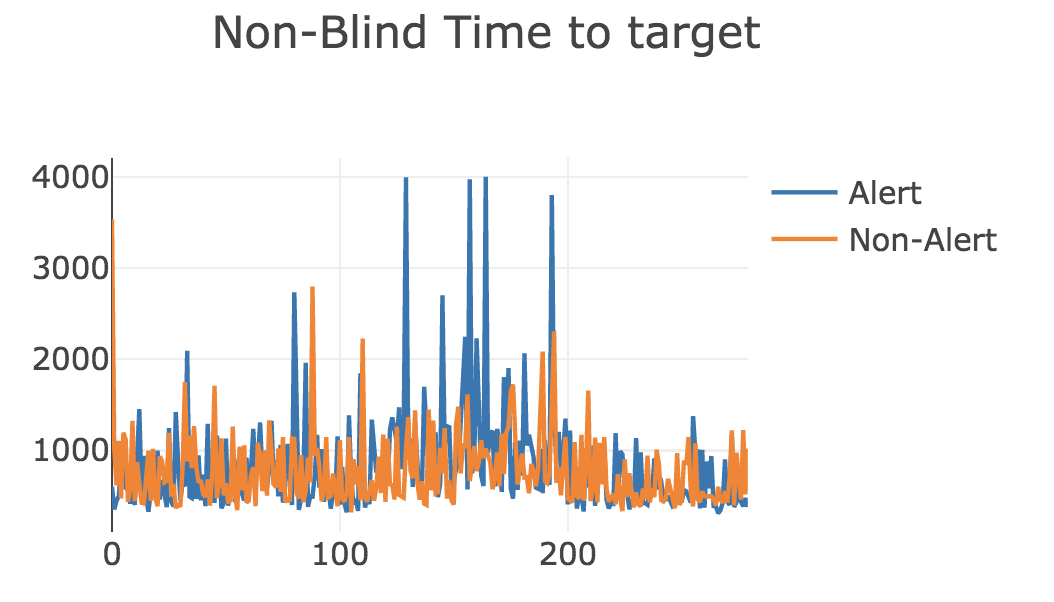
\includegraphics[width=1.2\textwidth]{images/nonblindtiming}
		\decoRule
  \end{subfigure}
  %
  \begin{subfigure}[b]{0.4\textwidth}
		\centering
    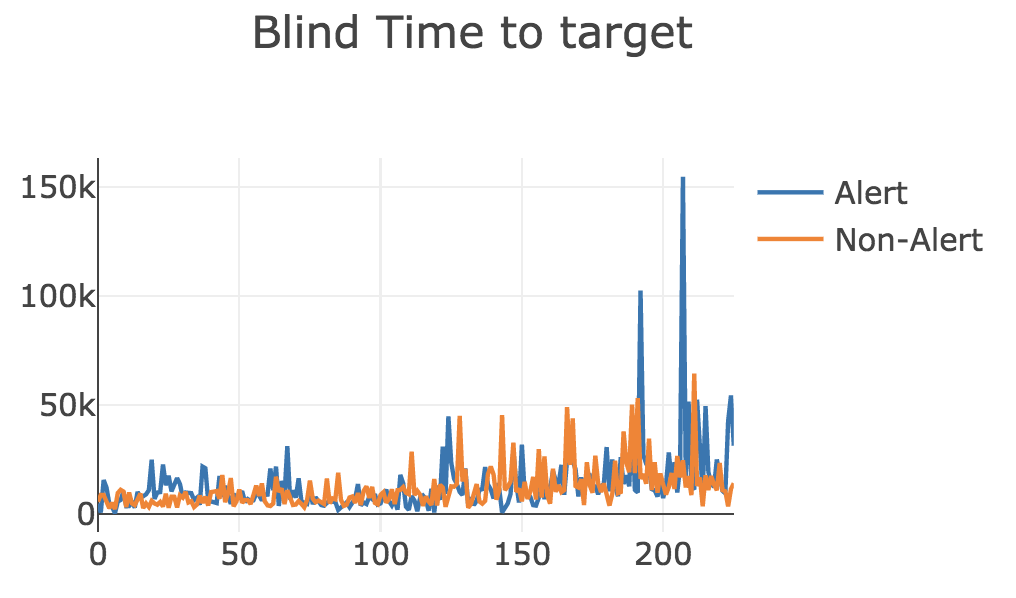
\includegraphics[width=1.2\textwidth]{images/blindtiming}
		\decoRule
  \end{subfigure}
	\caption[Phase 2 Timing Graph]{Time to target per round.}
	\label{fig:timing}
\end{figure}

Moving on to the second measurement, the distance from the center of each target to the successful click (which we can call target error) is illustrated across the parameters in Figure~\ref{fig:p2error}

\begin{figure}[h]
	\centering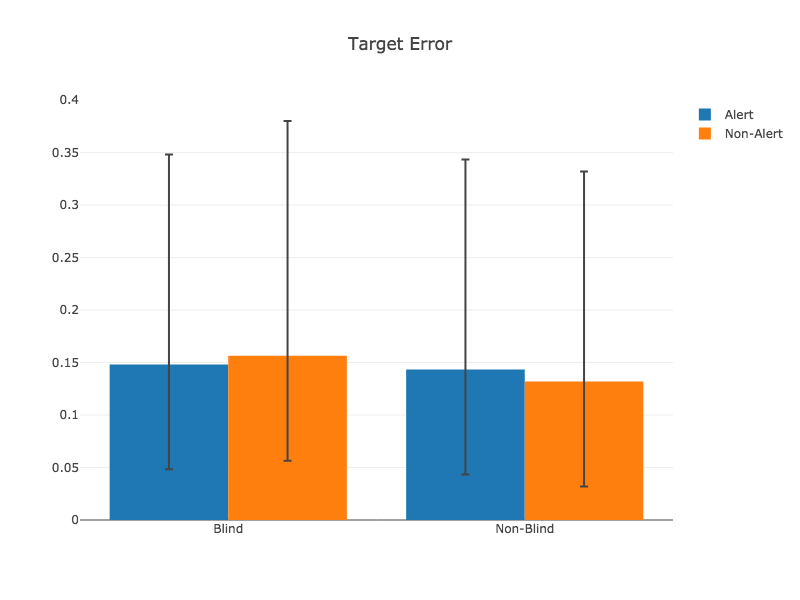
\includegraphics[width=1\linewidth]{images/distancetotarget}
	\decoRule
	\caption[Phase 2 Target Error]{Average Target Error.}
	\label{fig:p2error}
\end{figure}

From the graph, it doesn't seem that the presence of the alert variable has a strong effect on the target error. This is surprising as many participants had reported that they felt ``less accurate'' if the alert was given, since they would click much sooner and closer to the edges of a target. What is also interesting is that what little effect there is on the cumulative average is affected by whether the participants are blindfolded. It is very likely within the margin of error, as ANOVA (Figure~\ref{tab:p2erroranova}) fails to report any significance in the effect of the alert variable. It does however, place the effect of blindfolding as significant ($p < 1.0 \times 10^{-4}$, as expected) along with the interaction of the two variables. The true cause of this interaction is unknown, and as in the prior case further study is needed.

\begin{table}
	\centering
	\begin{tabular}{c|cccc}
		\toprule
		Effect & Sum Squares & dF & F & p\\
		\midrule
		Alert & 0.000336 & 1.0 & 0.058371 & 0.809125\\
		Blind & 0.086352 & 1.0 & 14.995669 & 0.000113\\
		Alert:Blind & 0.038955 & 1.0 & 6.764772 & 0.009396\\
		Residual & 7.975467 & 1385.0 & - & -\\
		\bottomrule
	\end{tabular}
	\caption[Phase 1 Target Error ANOVA]{ANOVA results for target error.}
	\label{tab:p2erroranova}
\end{table}

Further investigating the myriad interactions here, let's group results by individual. Figure~\ref{fig:p2individuals} shows a much clearer picture of how each individual performs against the variables as they change. Here we can see that the communal indicators are clearly misaligned with individual outcomes when the alert variable is introduced. In fact, the choice of individual clearly seems significant in determining how the alert variable affects the results.

\begin{figure}[h]
	\centering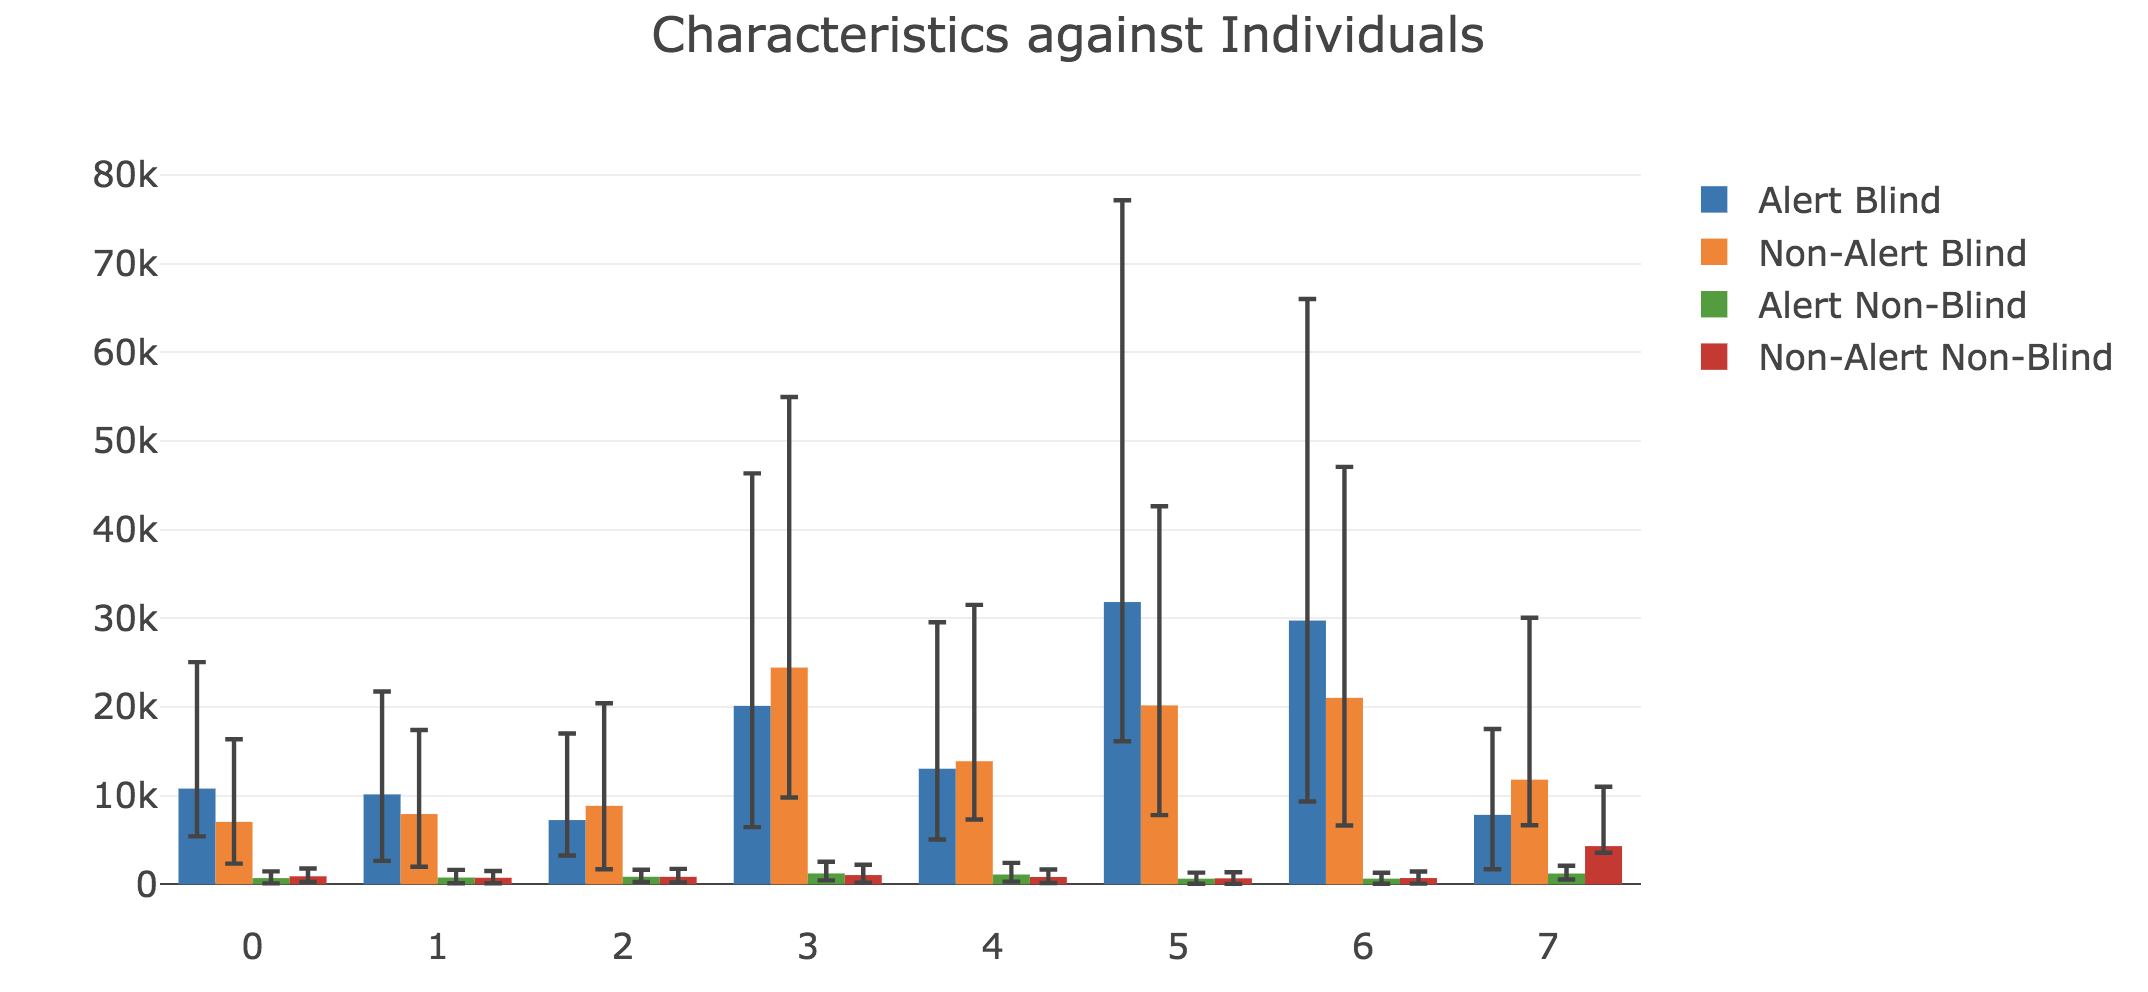
\includegraphics[width=1\linewidth]{images/individuals}
	\decoRule
	\caption[Phase 2 Individual Timing]{Timing and variables grouped against individuals.}
	\label{fig:p2individuals}
\end{figure}

\section{Discussion}

While a number of insights can be gleaned from the results gathered here, the strongest one is that increasing the number of dimensions merits a scaling-up of the sample size almost as much, perhaps even more so than the number of independent variables being modified. The uncertainty involved in human learning makes evaluating the effectiveness of more complex systems a challenging task. In reference to the related work that we have covered, it is clear that a mathematical model for determining sample size \textit{relative} to the complexity of the transmission protocol needs to be developed. However, the nature of the tasks used in the experiments here, which modify feedback latency, number of vectors, overall bandwidth and the measurements therein present a good framework against which to evaluate future work.

That being said, a few insights found in conducting the experiments that explain the behavior of the system can be laid out.

\subsection{Training}

In a sensory substitution module that aims to use neuroplasticity as a way of reconfiguring senses, much importance is placed on the participants being able to intuitively grasp the information being provided. In both the experiments conducted, I was surprised by the effect training time had on the performance of an individual, and in unexpected ways. Person 0 (from Figure~\ref{fig:p2individuals}) was aquainted with the experiment for the first time, and had to leave within a minute of starting due to scheduling conflicts. When they returned the next day, their performance had remarkably improved despite there being no conscious recollection of trying to improve their score. Likewise, participants that spent the first of the randomized sessions without access to the alert variable tended to perform much better than those that didn't. As in Phase 1, there seems to be a direct correlation between training time and performance, and while this seems obvious from the premise none of the related work that was consulted seemed to make use of or measure this parameter.

In addition, a lack of training time can lead to haphazard results that defy analysis. The first minute or two of most participants' time (well beyond the session that is often allocated for `getting used to' an experiment) was spent devising strategies to improve performance. For example, one of the participants preferred to circle the pointer in ever-tightening concentric circles, preferring to feel for the shift in vector direction across the axes as opposed to identifying and following them. However, given long enough all participants began to develop and intuitive sense for the information and saw marked increase in performance.

In my opinion, there appeared to be a battle of the conscious desire to remember and strategise a good solution, against the intuitive learning that took place given enough time. However, this merits further discussion and study.

\subsection{Active vs. Passive information flow}

Something that seemed to influence the participants was the active nature of the feedback being given. Comparing across both experiments, Phase 1 utilized a passive information approach whereby following the right path resulted in no response from the system, where Phase 2 did the inverse. From conducting the experiments, participants reported to have a stronger preference for a system that only provided corrective input as opposed to a surplus of information. This was an unexpected discovery that I believe can aid in the development of sensory substitution systems, where a passive approach is often overlooked.

\subsection{Demographics}

Finally, such experiments could benefit from tighter control over the demographics. While this increases the effort on the researcher's part, variation across the participants in age, build, gender and even mental state seemed to have a strong effect on the responses garnered therein. From prior experience in Human Computer Interfaces, this was much more pronounced here than in interfaces that required only a conscious level of learning.

\section{Further Research}

Due to the limited resources and scope of this paper, there is much to be desired in further work. Understanding the cognitive cycles of learning and intuition seem to hold the key to building high-bandwidth systems that can replace or enhance entire senses. As a next step, experiments in understanding the relationship between individual makeup, training time and training modality might be in order. Longer training sessions with intermittent testing periods can help measure the change as the brain comes to accept the new sense and begin to process the new reality.

The design framework, experiment structure and measurement protocols described herein were built with extensibility in mind. Future work could involve building on top of the encoding protocols to facilitate better cognitive acceptance of the new sense, as well as using standard tests such as Fitts' across multiple interfaces to compare and contrast possible best practices.

Finally, within the modular components of the framework lie the possibility of integrating some form of learning algorithm to tailor responses in real-time. Participants responded best when a continuously varying feedback loop was established, and the measurements laid out in the results section can be used to fine-tune the signals in a way that this loop is made stronger. While this is definitely outside the scope of this work, it is what seems to me the natural progression of the science.

\section{Conclusion}

In this paper, new frameworks, metrics and experiments for performing sensory substitution were explored in a way that made use of new advances in technology. The investigations demonstrated the need for more such frameworks that can be generalized towards conveying information as opposed to being successful at a specific task. The experiments found that the effects were strongly related to the dimensionality of input data, as well as the particular encoding being used.

The experiments were successful in developing a complete framework that enabled users to replace--for the purposes of spatial navigation in two and three dimensions--an existing sense in a manner that lowered cognitive load and the possibility of sensory overload. This has applications in Robotic Surgery and information dense environments such as combat fighters, MMORPGS, and data processing.

The paper also put forth a number of metrics that expanded upon existing literature in a way that makes future work easier to compare and buiid on top of. Of the configurations tried, successful configurations by way of hardware design and software encoding were found that best suited sensory uptake, as well as provide a modular platform whose results pointed to continuous-feedback based haptic systems as a way of replacing and enhancing the umwelt.

%----------------------------------------------------------------------------------------
%	THESIS CONTENT - APPENDICES
%----------------------------------------------------------------------------------------

\appendix % Cue to tell LaTeX that the following "chapters" are Appendices

\chapter{Supporting material}

Interactive versions of the graphs used in this paper can be found at \href{https://plot.ly/~toonistic/}{https://plot.ly/~toonistic/}, along with the datasets used.

The code used in this experiment\footnote{Strictly of research quality and to be considered at best an alpha release.} along with detailed datasets and debug logs can be found at \href{https://github.com/hrishioa/goosebumps}{https://github.com/hrishioa/goosebumps}.

A video of the experiment setup for Phase 1 is located on Youtube at \href{https://youtu.be/5U9C2m8akOc}{https://youtu.be/5U9C2m8akOc}.

% Include the appendices of the thesis as separate files from the Appendices folder
% Uncomment the lines as you write the Appendices

% % Appendix A

\chapter{Frequently Asked Questions} % Main appendix title

\label{AppendixA} % For referencing this appendix elsewhere, use \ref{AppendixA}

\section{How do I change the colors of links?}

The color of links can be changed to your liking using:

{\small\verb!\hypersetup{urlcolor=red}!}, or

{\small\verb!\hypersetup{citecolor=green}!}, or

{\small\verb!\hypersetup{allcolor=blue}!}.

\noindent If you want to completely hide the links, you can use:

{\small\verb!\hypersetup{allcolors=.}!}, or even better: 

{\small\verb!\hypersetup{hidelinks}!}.

\noindent If you want to have obvious links in the PDF but not the printed text, use:

{\small\verb!\hypersetup{colorlinks=false}!}.

%\include{Appendices/AppendixB}
%\include{Appendices/AppendixC}

%----------------------------------------------------------------------------------------
%	BIBLIOGRAPHY
%----------------------------------------------------------------------------------------

\printbibliography[heading=bibintoc]

%----------------------------------------------------------------------------------------

\end{document}
